\documentclass{beamer}	
\mode<presentation>
 
\usepackage{pdfpages}
\usepackage{fancyvrb}
\usepackage{chemarr}

\usepackage{amsmath}		%% mathematics typesetting
\usepackage{amssymb}
 
\usepackage{listings}   %% code listings

\usepackage{hyperref}

\usepackage{booktabs}

\usepackage{CJKutf8} %% typeset Chinese characters

\usepackage{pdfpages}

% Color and Theme. Can be changed. However, this one's quite nice.
\usetheme{Madrid}
\definecolor{theme}{rgb}{0.49,0.65,0.57}
\usecolortheme[named=theme]{structure}



%%  Title information
\title[Nozizeption]{Nozizeption und Schmerz}
\author[melanie.stefan@ed.ac.uk]{Melanie Stefan - melanie.stefan@ed.ac.uk}
\date{25.8.2021}


% Table of contents to pop up at the beginning of each section
\AtBeginSection[]
{
  \begin{frame}<beamer>
    \frametitle{Outline}
    \tableofcontents[currentsection,currentsubsection]
  \end{frame}
}
 
\beamertemplatenavigationsymbolsempty

\begin{document}
 

{
  \usebackgroundtemplate{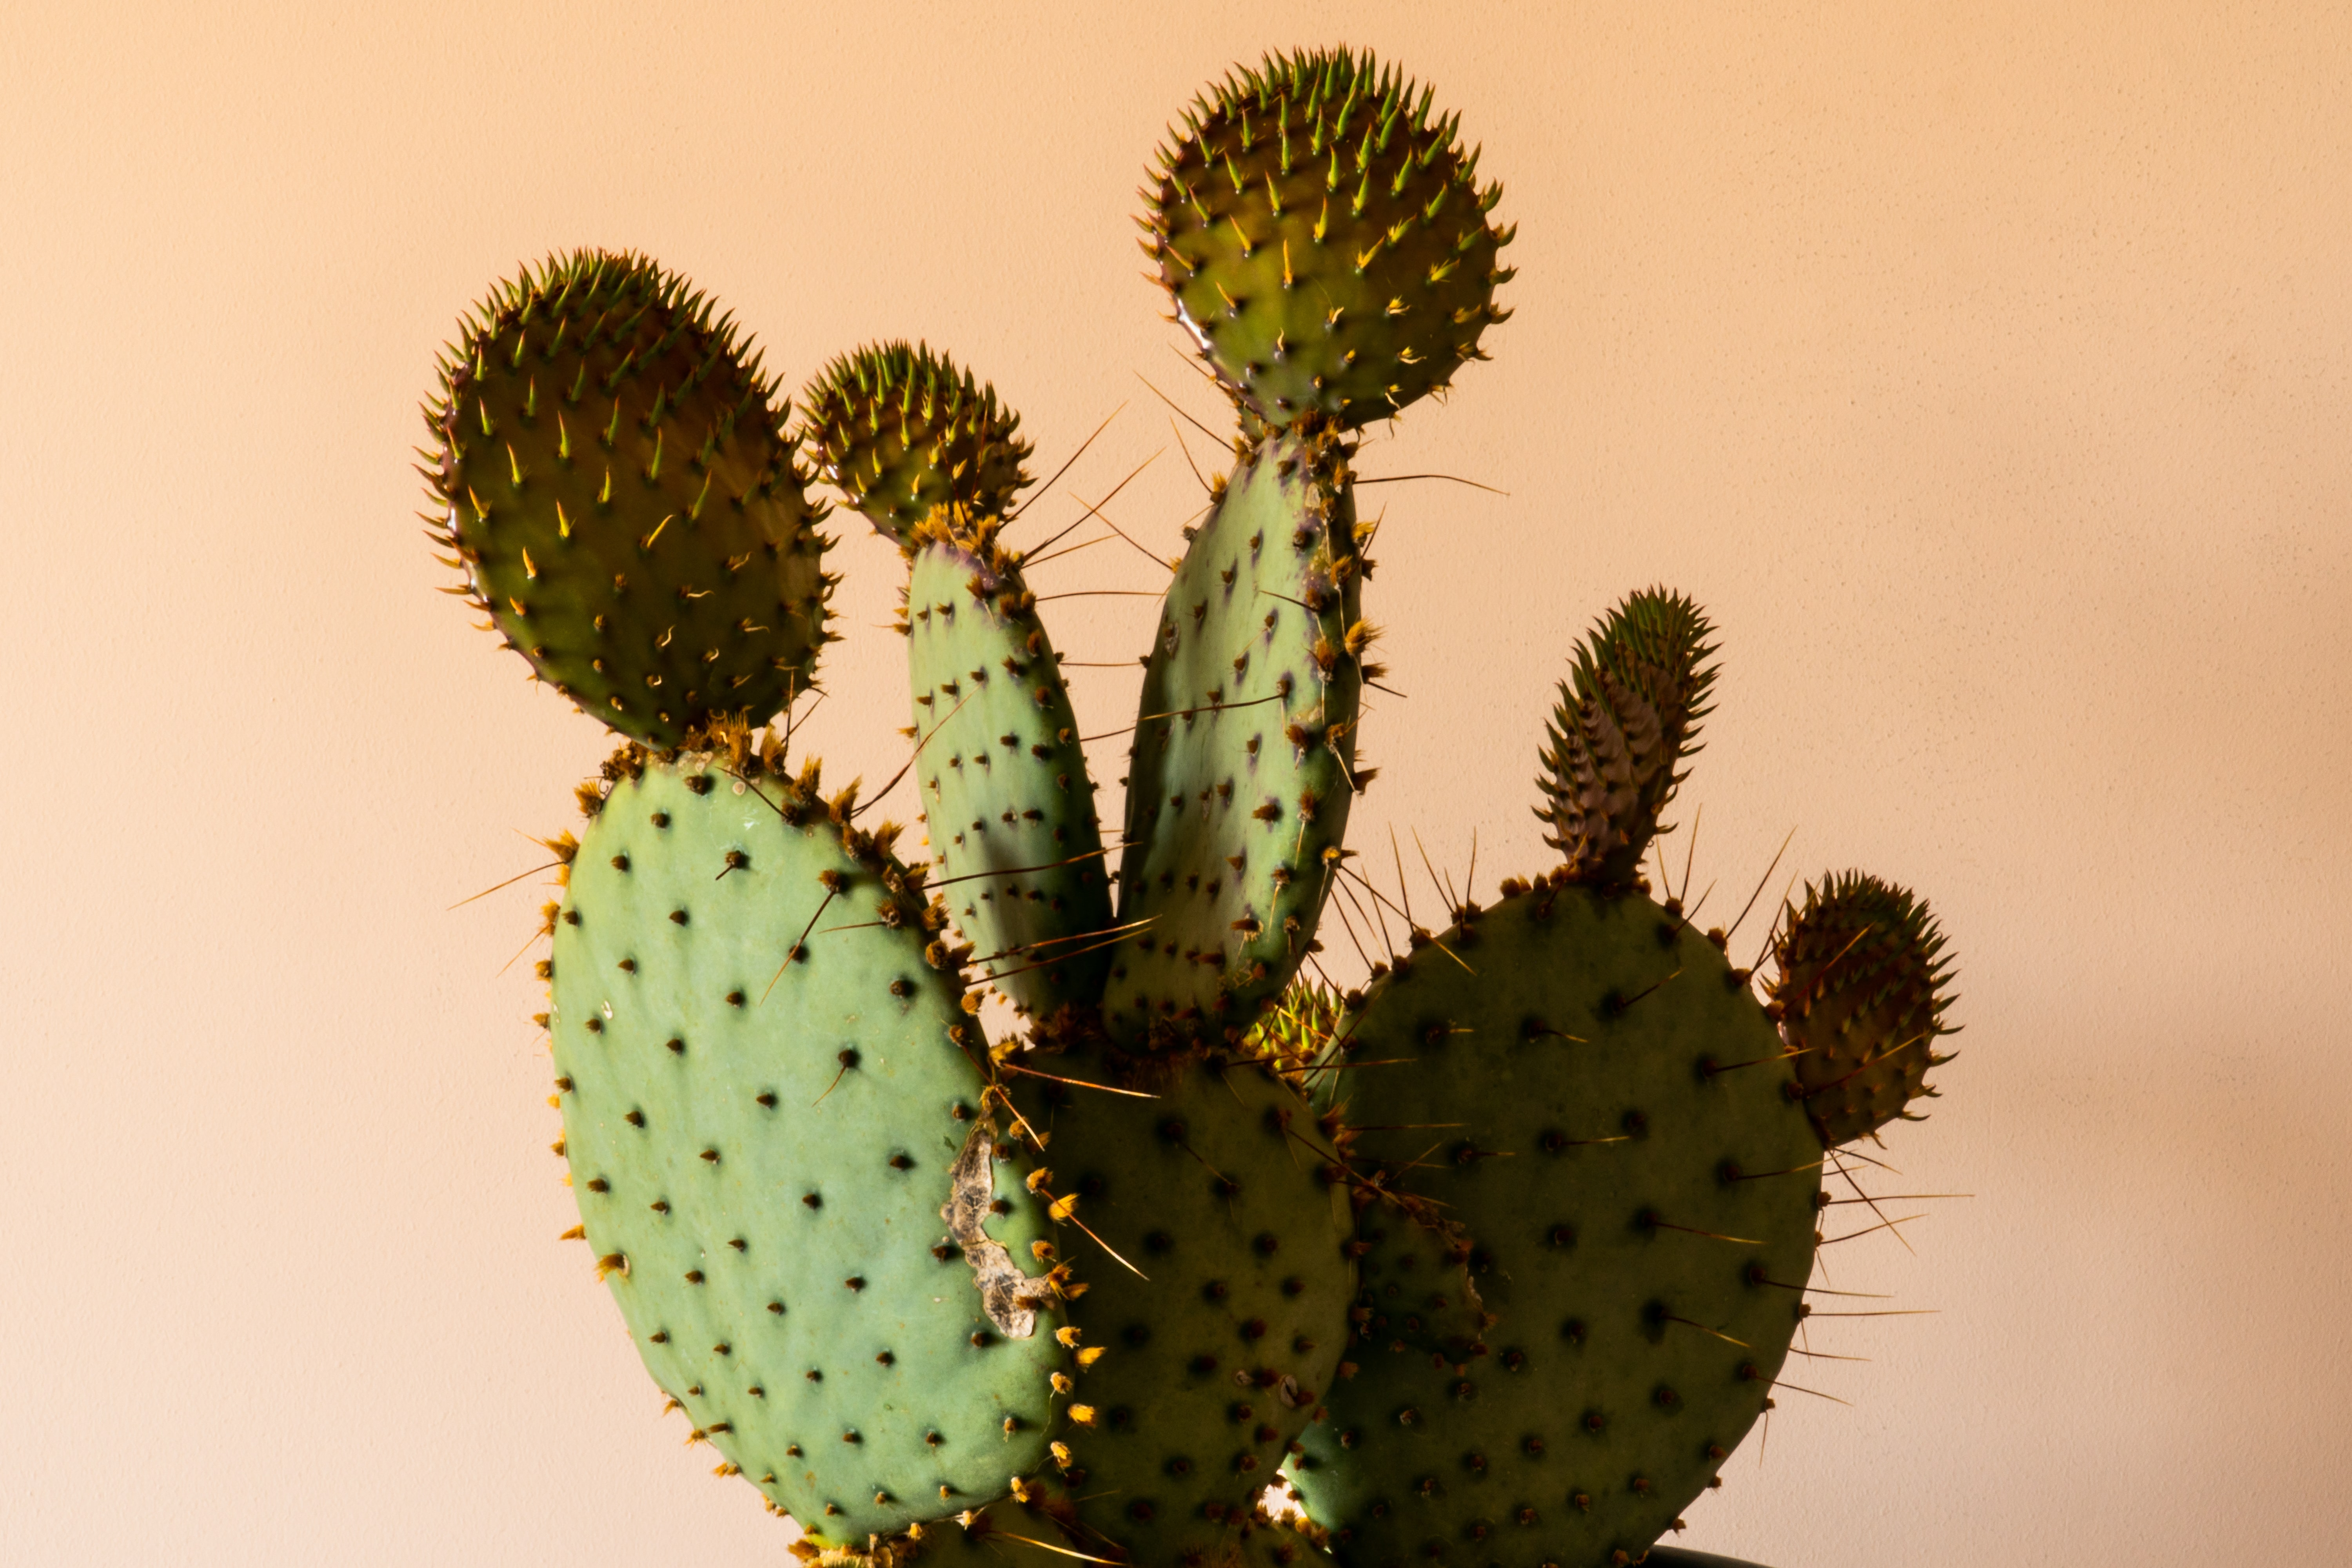
\includegraphics[width=1.4\paperwidth]{/home/melanie/Work/pictures/metaphore/cactus.jpg}}
\begin{frame}[plain]

% \maketitle 

\begin{Large}\textbf{Nozizeption und Schmerz}
\end{Large} \\[3cm]

Melanie Stefan, \\

melanie.stefan@ed.ac.uk \\


25.8.2021 

\vfill


\end{frame}
}

%% Hook: 
\begin{frame}
\frametitle{Was Sie schon immer über Schmerz wissen wollten \dots}
\pause

\begin{itemize}
\item
Warum ist auf Sonnenbrand alles schmerzhaft, sogar ein T-Shirt?
\item
Wie funktioniert eigentlich Aspirin? 
\item
Warum können Schmerzen im Arm ein Anzeichen von Herzinfarkt sein? 
\item
Warum kann man bei Schmerzen schlecht schlafen? 
\item
Warum tut es weh, besonders scharfe Chilis zu essen?
\item
Warum haben manche Menschen nie Schmerzen? Und andere dauernd?
\item
Warum hilft Bewegung bei Regelschmerzen? 
\item
Wie funktionieren Phantomschmerzen?  
\item
\dots 
\end{itemize}


\end{frame}



%% TLIA

\begin{frame}
\frametitle{Wie der Schmerz ins Rückenmark kommt}

\pause 
\begin{center}
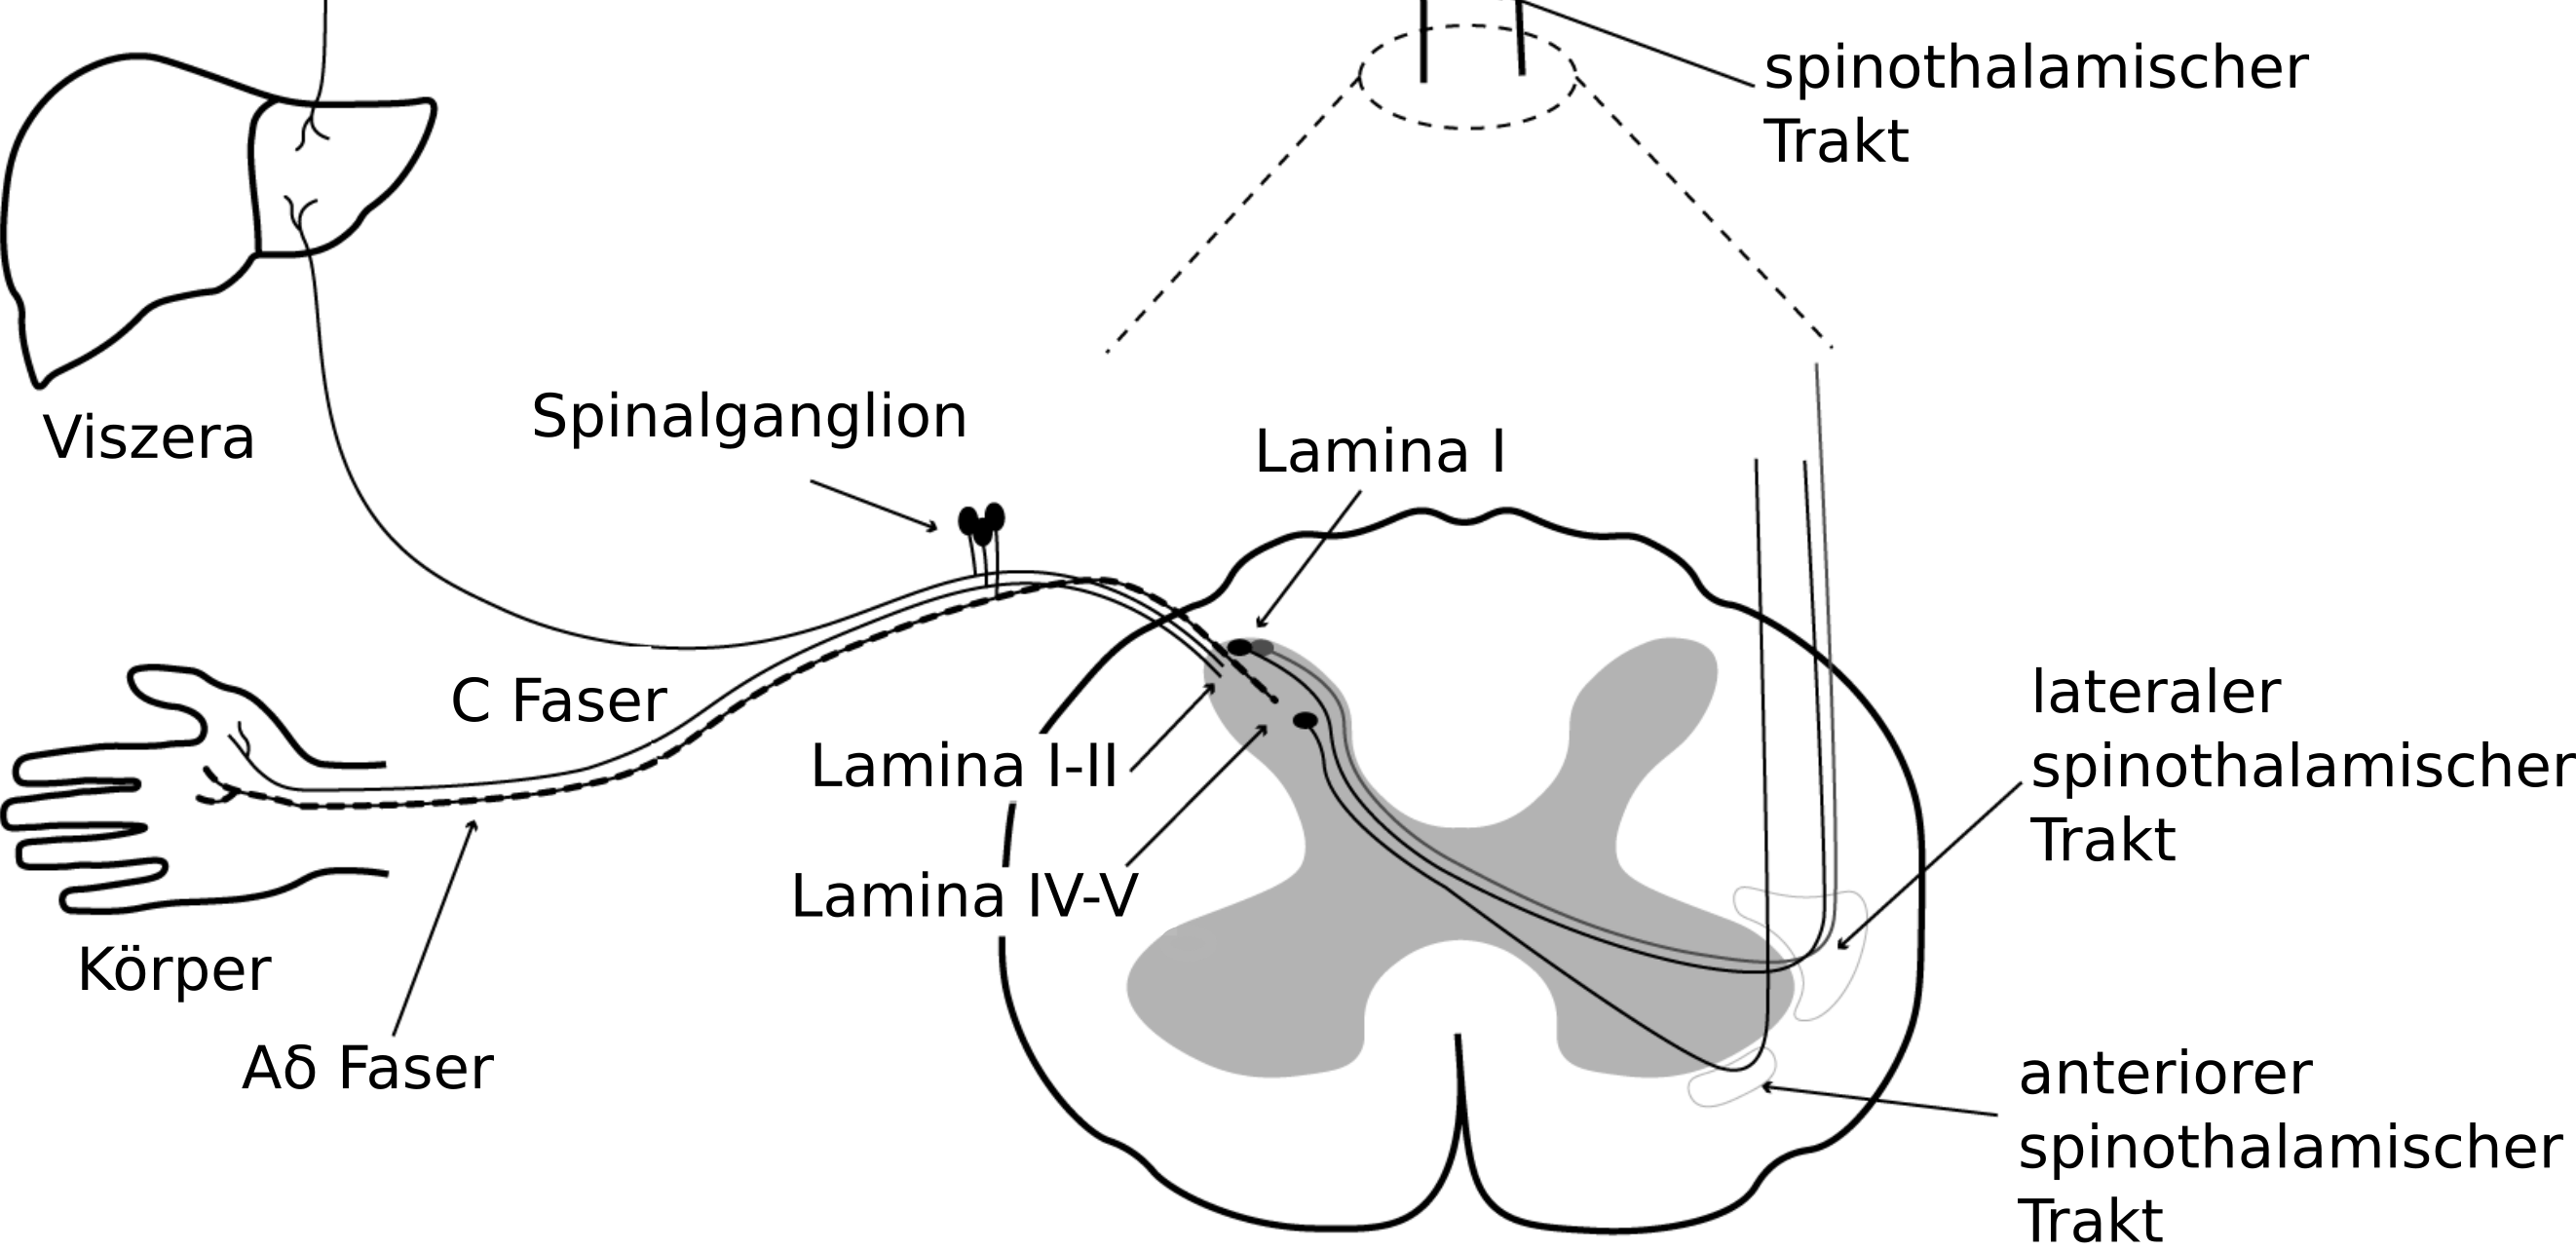
\includegraphics[width=\textwidth]{/home/melanie/Work/pictures/brain/Schmerz_aufsteigend_bis_Rueckenmark.png}
\end{center}

\end{frame}


%% Learning Objectives
 \begin{frame}
\frametitle{Lernziele}


\begin{block}{Nach dieser Vorlesung werden Sie folgendes können:}



\begin{itemize}
\item
Den allgemeinen Weg des Schmerzreizes vom Nozizeptor bis ins Gehirn beschreiben
\item
Die drei Arten von Nozizeption aufzählen und beschreiben
\item
Erklären, wie Schmerz-Rezeptoren aktiviert werden
\item
Modifikatoren von Schmerz-Rezeptoren benennen und erklären
\item
Erklären, was schnellen von langsamem Schmerz unterscheidet
\item
Erklären, was  übertragener Schmerz ist und wann er vorkommt
\end{itemize}


\end{block}


\end{frame}


%% Main Body


%% Überblick Schmerz ins Hirn
\begin{frame}
\frametitle{Wie der Schmerz ins Hirn kommt}

\begin{center}
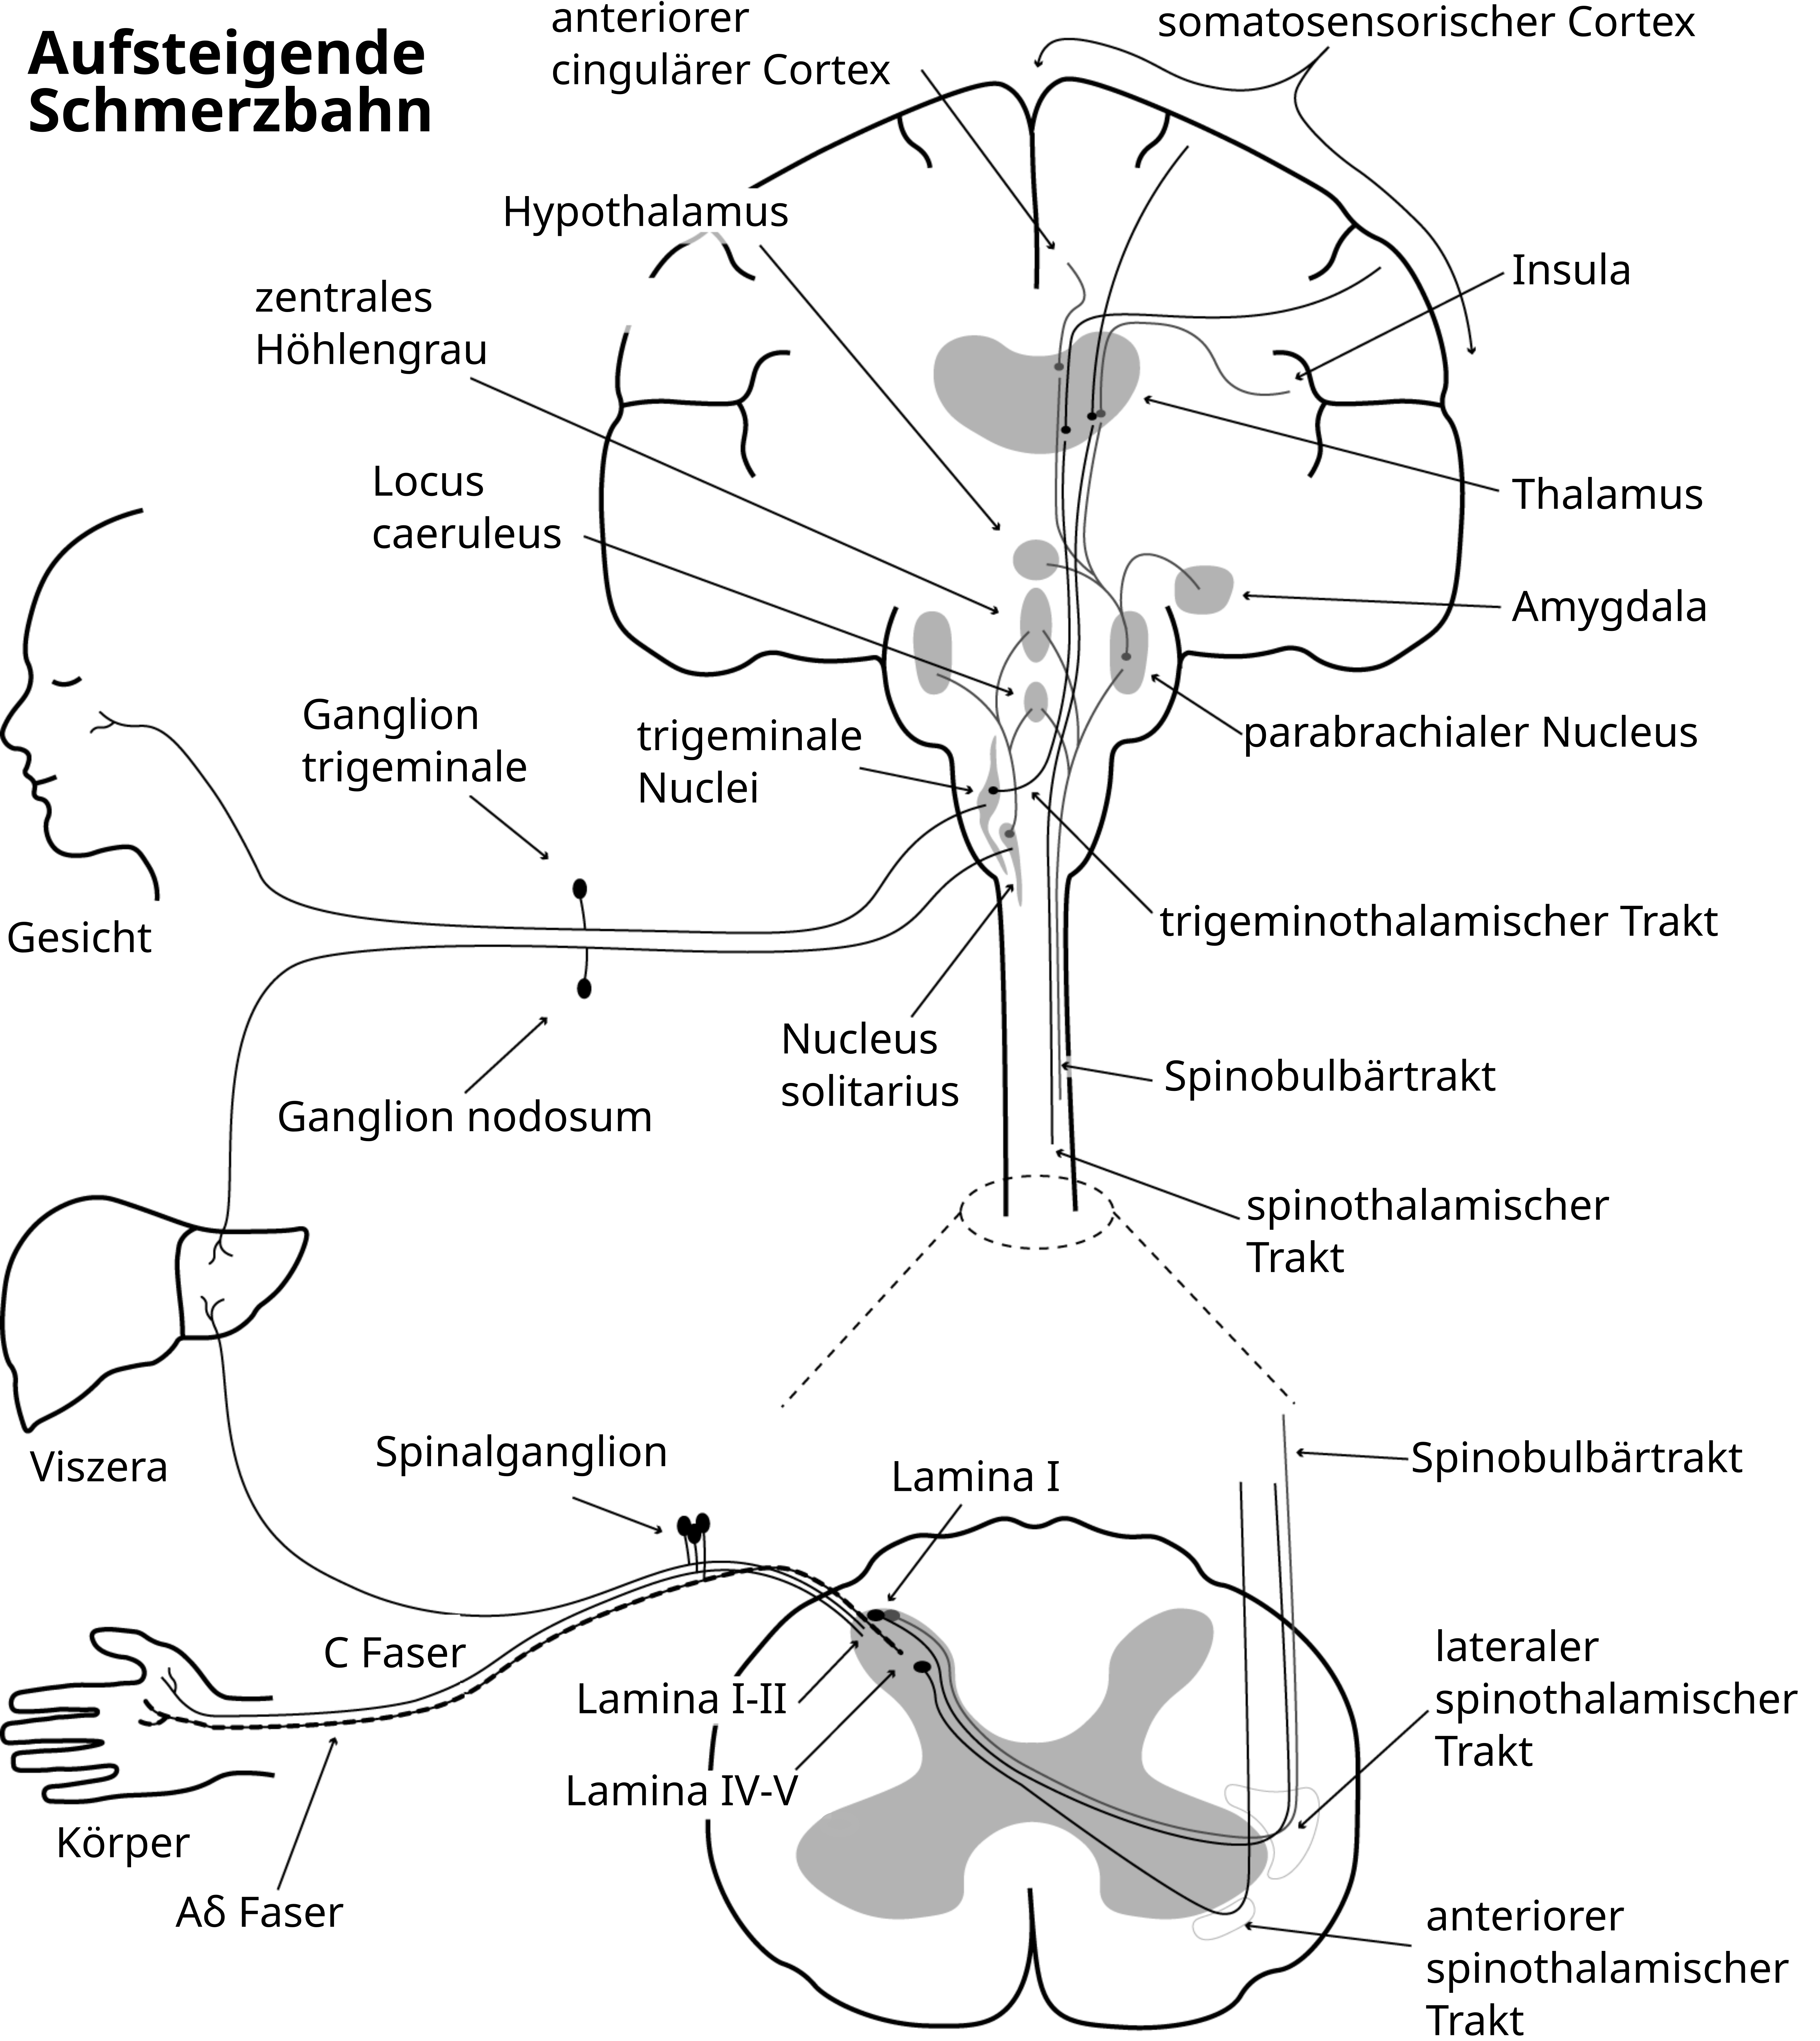
\includegraphics[width=0.5\textwidth]{/home/melanie/Work/pictures/brain/Schmerz_aufsteigend.png}
\end{center}

\end{frame}



%% Nozizeptoren: mechano, thermo, chemo
\begin{frame}
\frametitle{Nozizeptoren}


\begin{center}
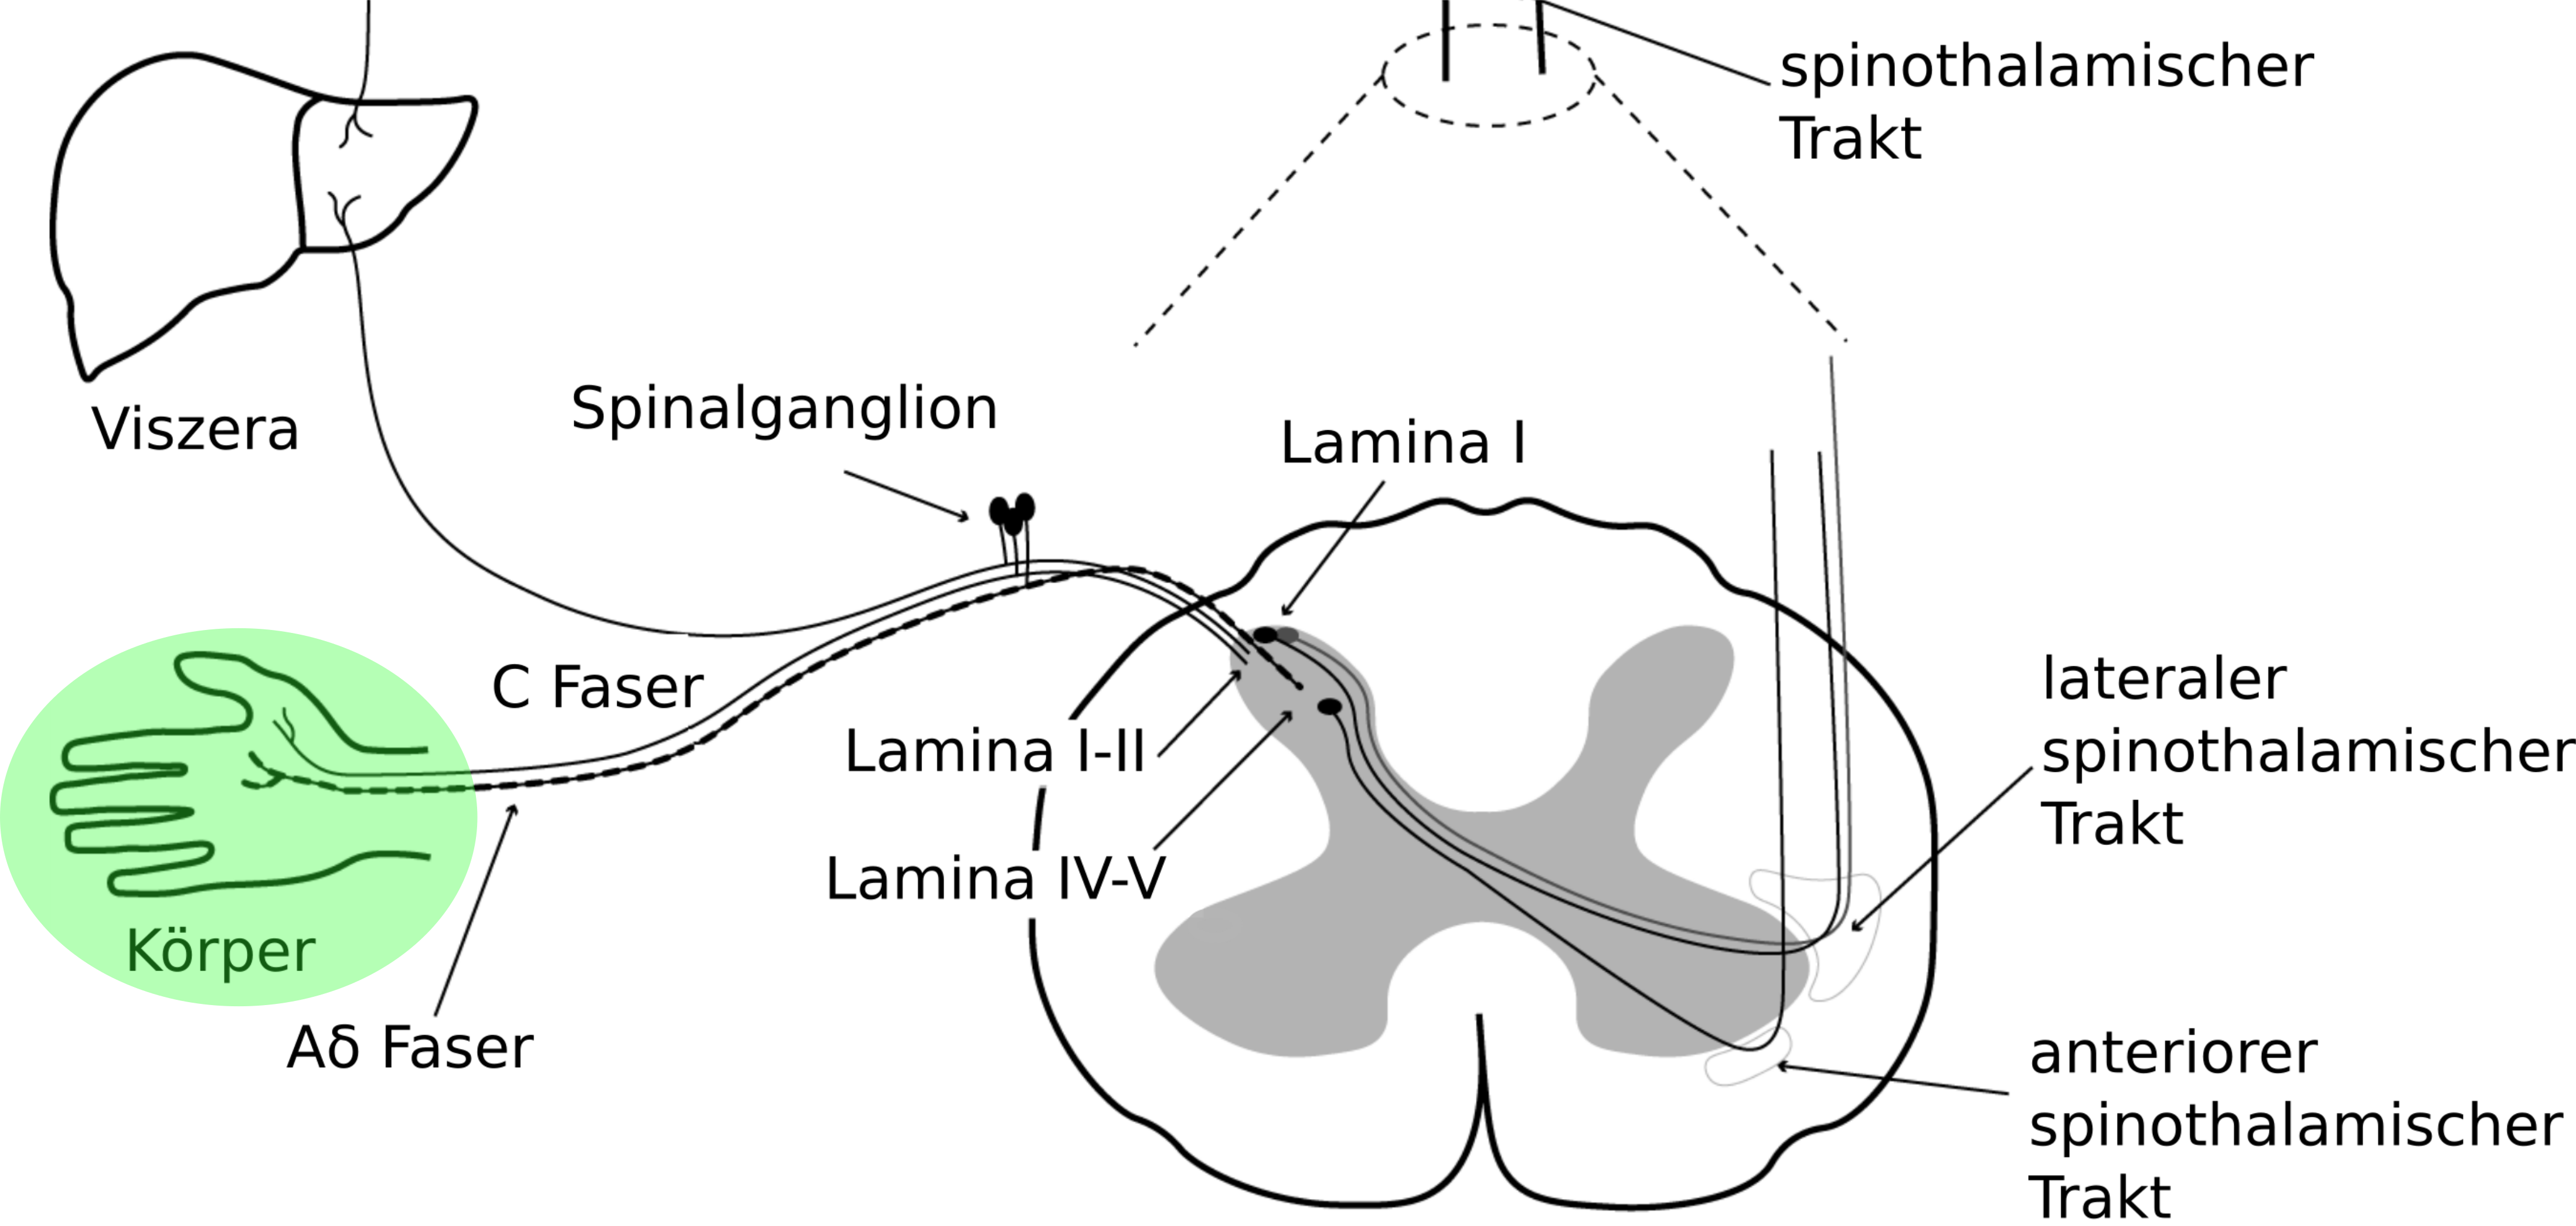
\includegraphics[width=\textwidth]{/home/melanie/Work/pictures/brain/Schmerz_aufsteigend_bis_Rueckenmark_Nozizeptor.png}
\end{center}

Nozizeptoren (Schmerz-Empfänger) sind freie Nervenendigungen. 
 
\end{frame}


\begin{frame}
\frametitle{Nozizeptoren}

Drei Arten von Schmerz können wahrgenommen werden:

\begin{itemize}
\item
Mechanisch (Verformung im Gewebe)
\item
Thermisch (Hitze oder Kälte)
\item
Chemisch (Körpereigene Substanzen, die z.B. bei Gewebeschäden freigesetzt werden)
\end{itemize}

\pause 
Viele Nozizeptoren sind \textcolor{theme}{polymodal}, können also mehrere Arten von Schmerz empfangen. 

\end{frame}



\begin{frame}
\frametitle{Molekulare Mechanismen}

\begin{columns}[c]

\begin{column}{7cm}
\begin{itemize}
\item
In der Membran von Nozizeptoren sitzen verschiedene Arten von Kationenkanälen 
\item
Die Ionenkanäle sind an Rezeptoren gekoppelt; Aktivierung des Rezeptors öffnet den Kanal
\end{itemize}



\end{column}

\begin{column}{5cm}
\begin{center}
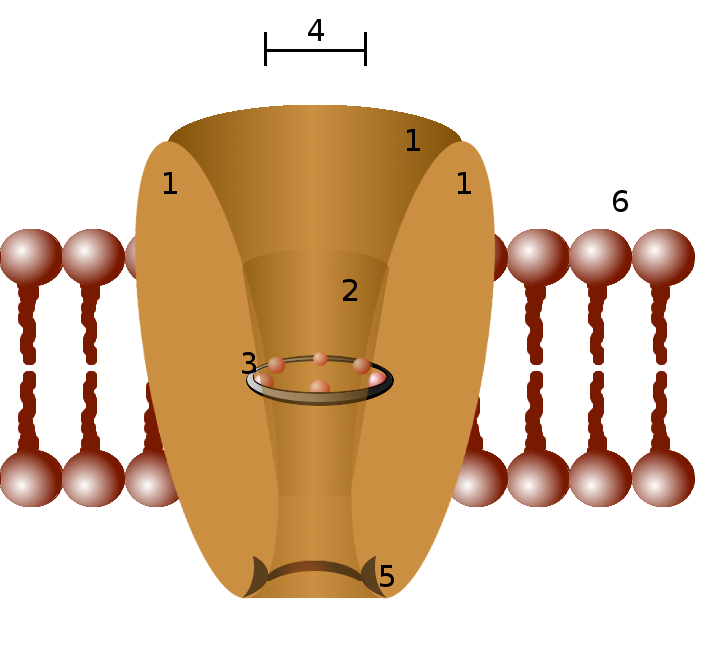
\includegraphics[width=0.7\textwidth]{/home/melanie/Work/pictures/physiology/Ion_channel.png}
\end{center}
\end{column}

\end{columns}

\begin{itemize}
\item
Kationen kommen in die Zelle und generieren ein Aktionspotential 
\item
Je nach Reiz unterschiedliche Rezeptoren und Kanäle und unterschiedliche Mechanismen (mechanisch, thermisch, chemisch)
\item
Manchmal wirken mehrere mögliche Reize auf denselben Rezeptor
\end{itemize}


\end{frame}


\begin{frame}
\frametitle{Beispiel: TRPV1}

\begin{center}
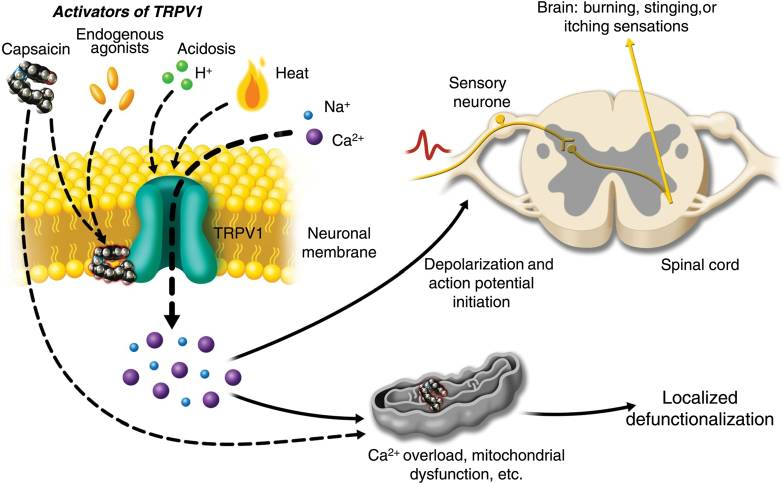
\includegraphics[width=\textwidth]{/home/melanie/Work/pictures/physiology/Activation_of_TRPV1_by_capsaicin.jpg}
\end{center}



\end{frame}

%% Nozizeptor-Aktivatoren: Substance P, Bradikynin


\begin{frame}
\frametitle{Manche Neuropeptide lösen chemische Nozizeption über GPCR aus}


Manche Kationenkanäle für die Schmerzwahrnehmung können durch Phosphorylierung (im innerzellulären Teil) aktiviert werden. 


\begin{center}
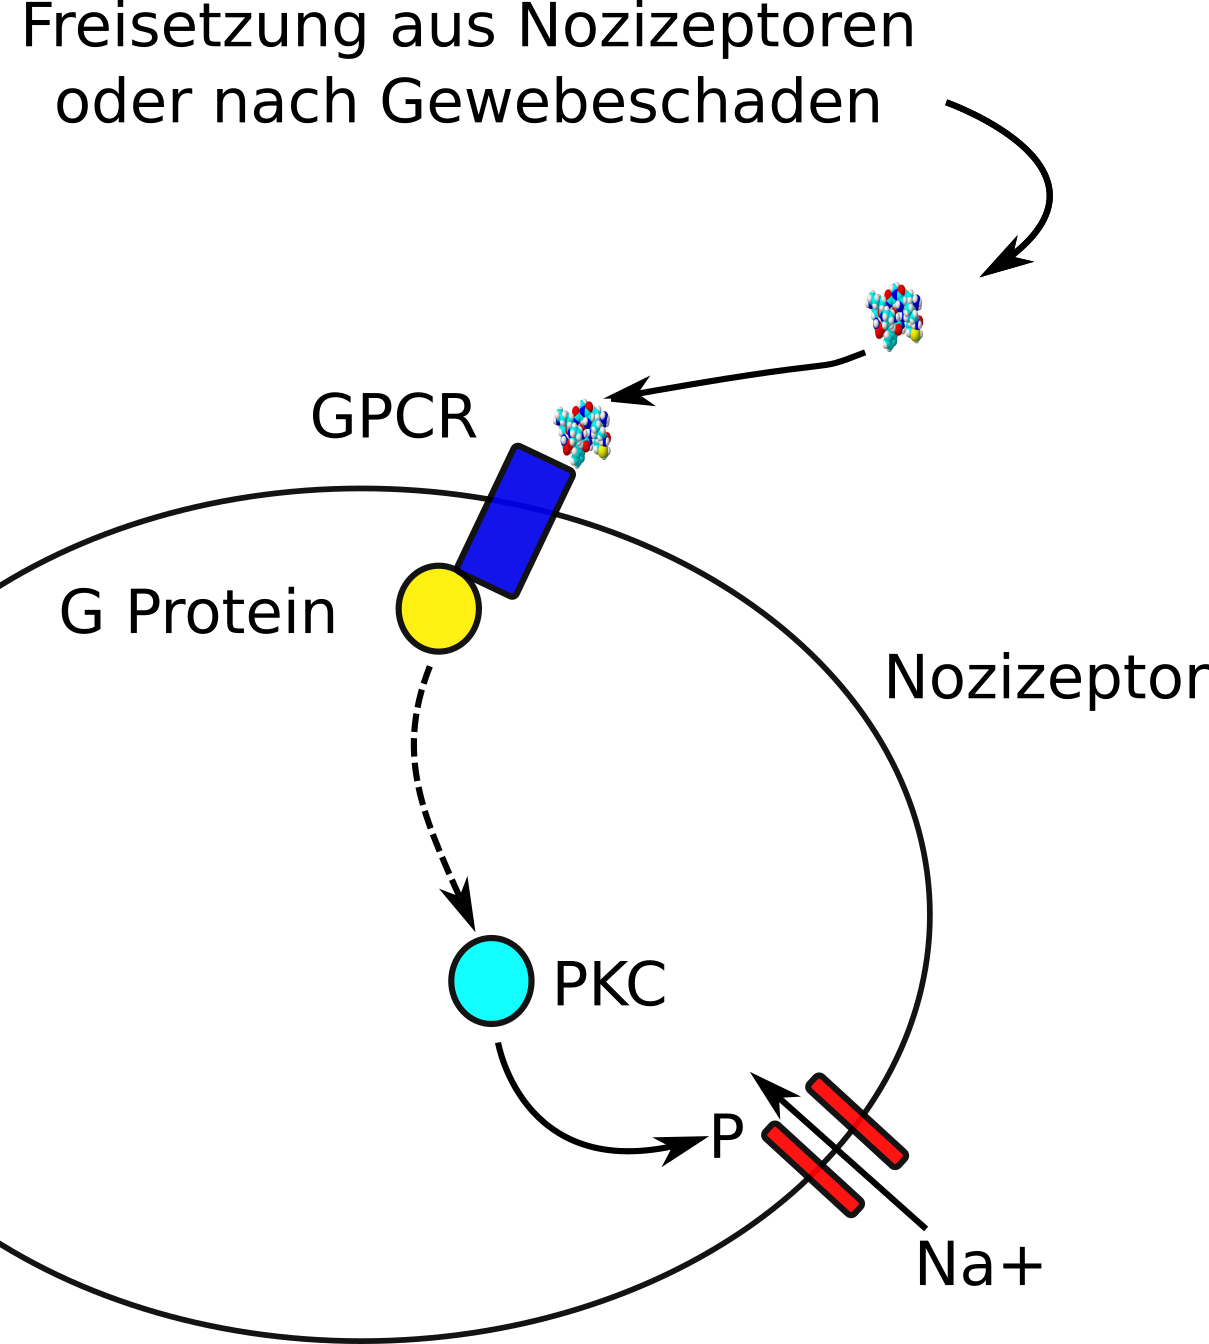
\includegraphics[width=0.4\textwidth]{/home/melanie/Work/pictures/brain/nozizeptive_neuropeptide.png}
\end{center}



\end{frame}



\begin{frame}
\frametitle{Manche Neuropeptide lösen chemische Nozizeption über GPCR aus}


\begin{itemize}
\item 
Schmerz-modifizierende Substanz wird (extrazellulär) freigesetzt und trifft auf eine Nervenzelle
\item
Die Substanz bindet an einen G-Protein-gekoppelten Rezeptor (GPCR)
\item
Dies führt zur Aktivierung von G-Proteinen innerhalb der Nervenzelle und in weiterer Folge Aktivierung von Protein Kinase C (PKC)
\item
PKC phosphoryliert einen Natrium-Kanal, der dadurch geöffnet wird
\end{itemize}


\end{frame}


\begin{frame}


\frametitle{Bradykinin}

\begin{itemize}
\item
Kleines Neuropeptid (9 Aminosäuren)
\item
Wird bei Gewebeschäden freigesetzt 
\item
Verursacht eine Erweiterung der Blutgefäße und trägt damit zum Entzündungsgeschehen bei
\item
Aktiviert Nozizeptor durch Binden an einen GPCR
\end{itemize}


\end{frame}


\begin{frame}
\frametitle{Substanz P}

\begin{columns}[c]
\begin{column}{5cm}
\begin{itemize}
\item
Kleines Neuropeptid (11 Aminosäuren)
\item
Wird bei Schmerz aus Nozizeptoren freigesetzt
\item
Aktiviert den NK-1 Rezeptor (NK1R)
\item
Wie Bradykinin am Entzündungsgeschehen beteiligt 
\item 
Funktioniert nicht nur als Aktivator, sondern auch als \textcolor{theme}{Modulator} der Schmerzwahrnehmung
\end{itemize}

\end{column}

\begin{column}{5cm}
\begin{center}
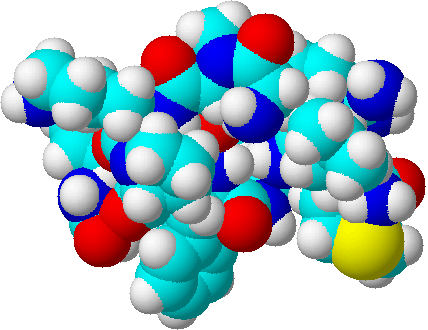
\includegraphics[width=0.7\textwidth]{/home/melanie/Work/pictures/physiology/Substance_P.png}
\end{center}
\end{column}
\end{columns}


\end{frame}


%% Nozizeptor-Modifikatoren (Hyperalgesie/Allodynie) - Substanz P, Prostaglandin

\begin{frame}
\frametitle{Nozizeptor-Modulatoren}

\begin{itemize}
\item
Nozizeptor-Modulatoren können einen Ionenkanal im Nozizeptor sensibilisieren.
\item
Der Ionenkanal wird dadurch nicht direkt aktiviert, aber seine Aktivierungsschwelle sinkt.
\end{itemize}

\begin{columns}[c]
\begin{column}{6.5cm}

\begin{itemize}
\item
Schmerzhafte Reize werden dadurch noch schmerzhafter (Hyperalgesie) \emph{und}

\item
Reize, die normalerweise nicht schmerzhaft sind (z.B. Berührung) können schmerzhaft werden (Allodynie)
\end{itemize}
\end{column}

\begin{column}{5cm}
\begin{center}
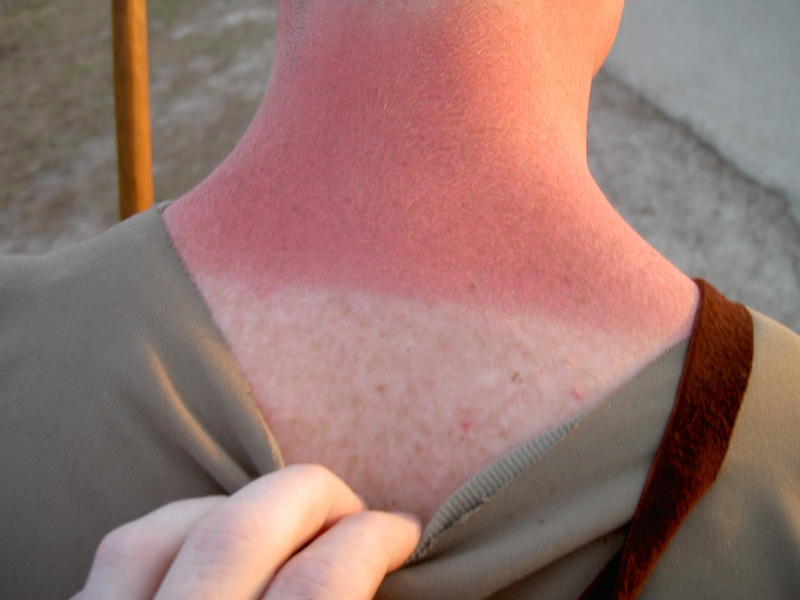
\includegraphics[width=\textwidth]{/home/melanie/Work/pictures/physiology/Sunburn.jpg}
\end{center}

\end{column}
\end{columns}

\end{frame}



\begin{frame}
\frametitle{Prostaglandin}

Prostaglandin entsteht bei Gewebeschaden aus dem Abbau von Phospholipiden in der Zellmembran

\pause

\begin{center}

\includegraphics[width=0.5\textwidth]{/home/melanie/Work/pictures/physiology/prostaglandin_synthese.png}
\end{center}



\end{frame}


%% Schneller und langsamer Schmerz
\begin{frame}
\frametitle{Weiterleitung über Nervenfasern}
 
\begin{center}
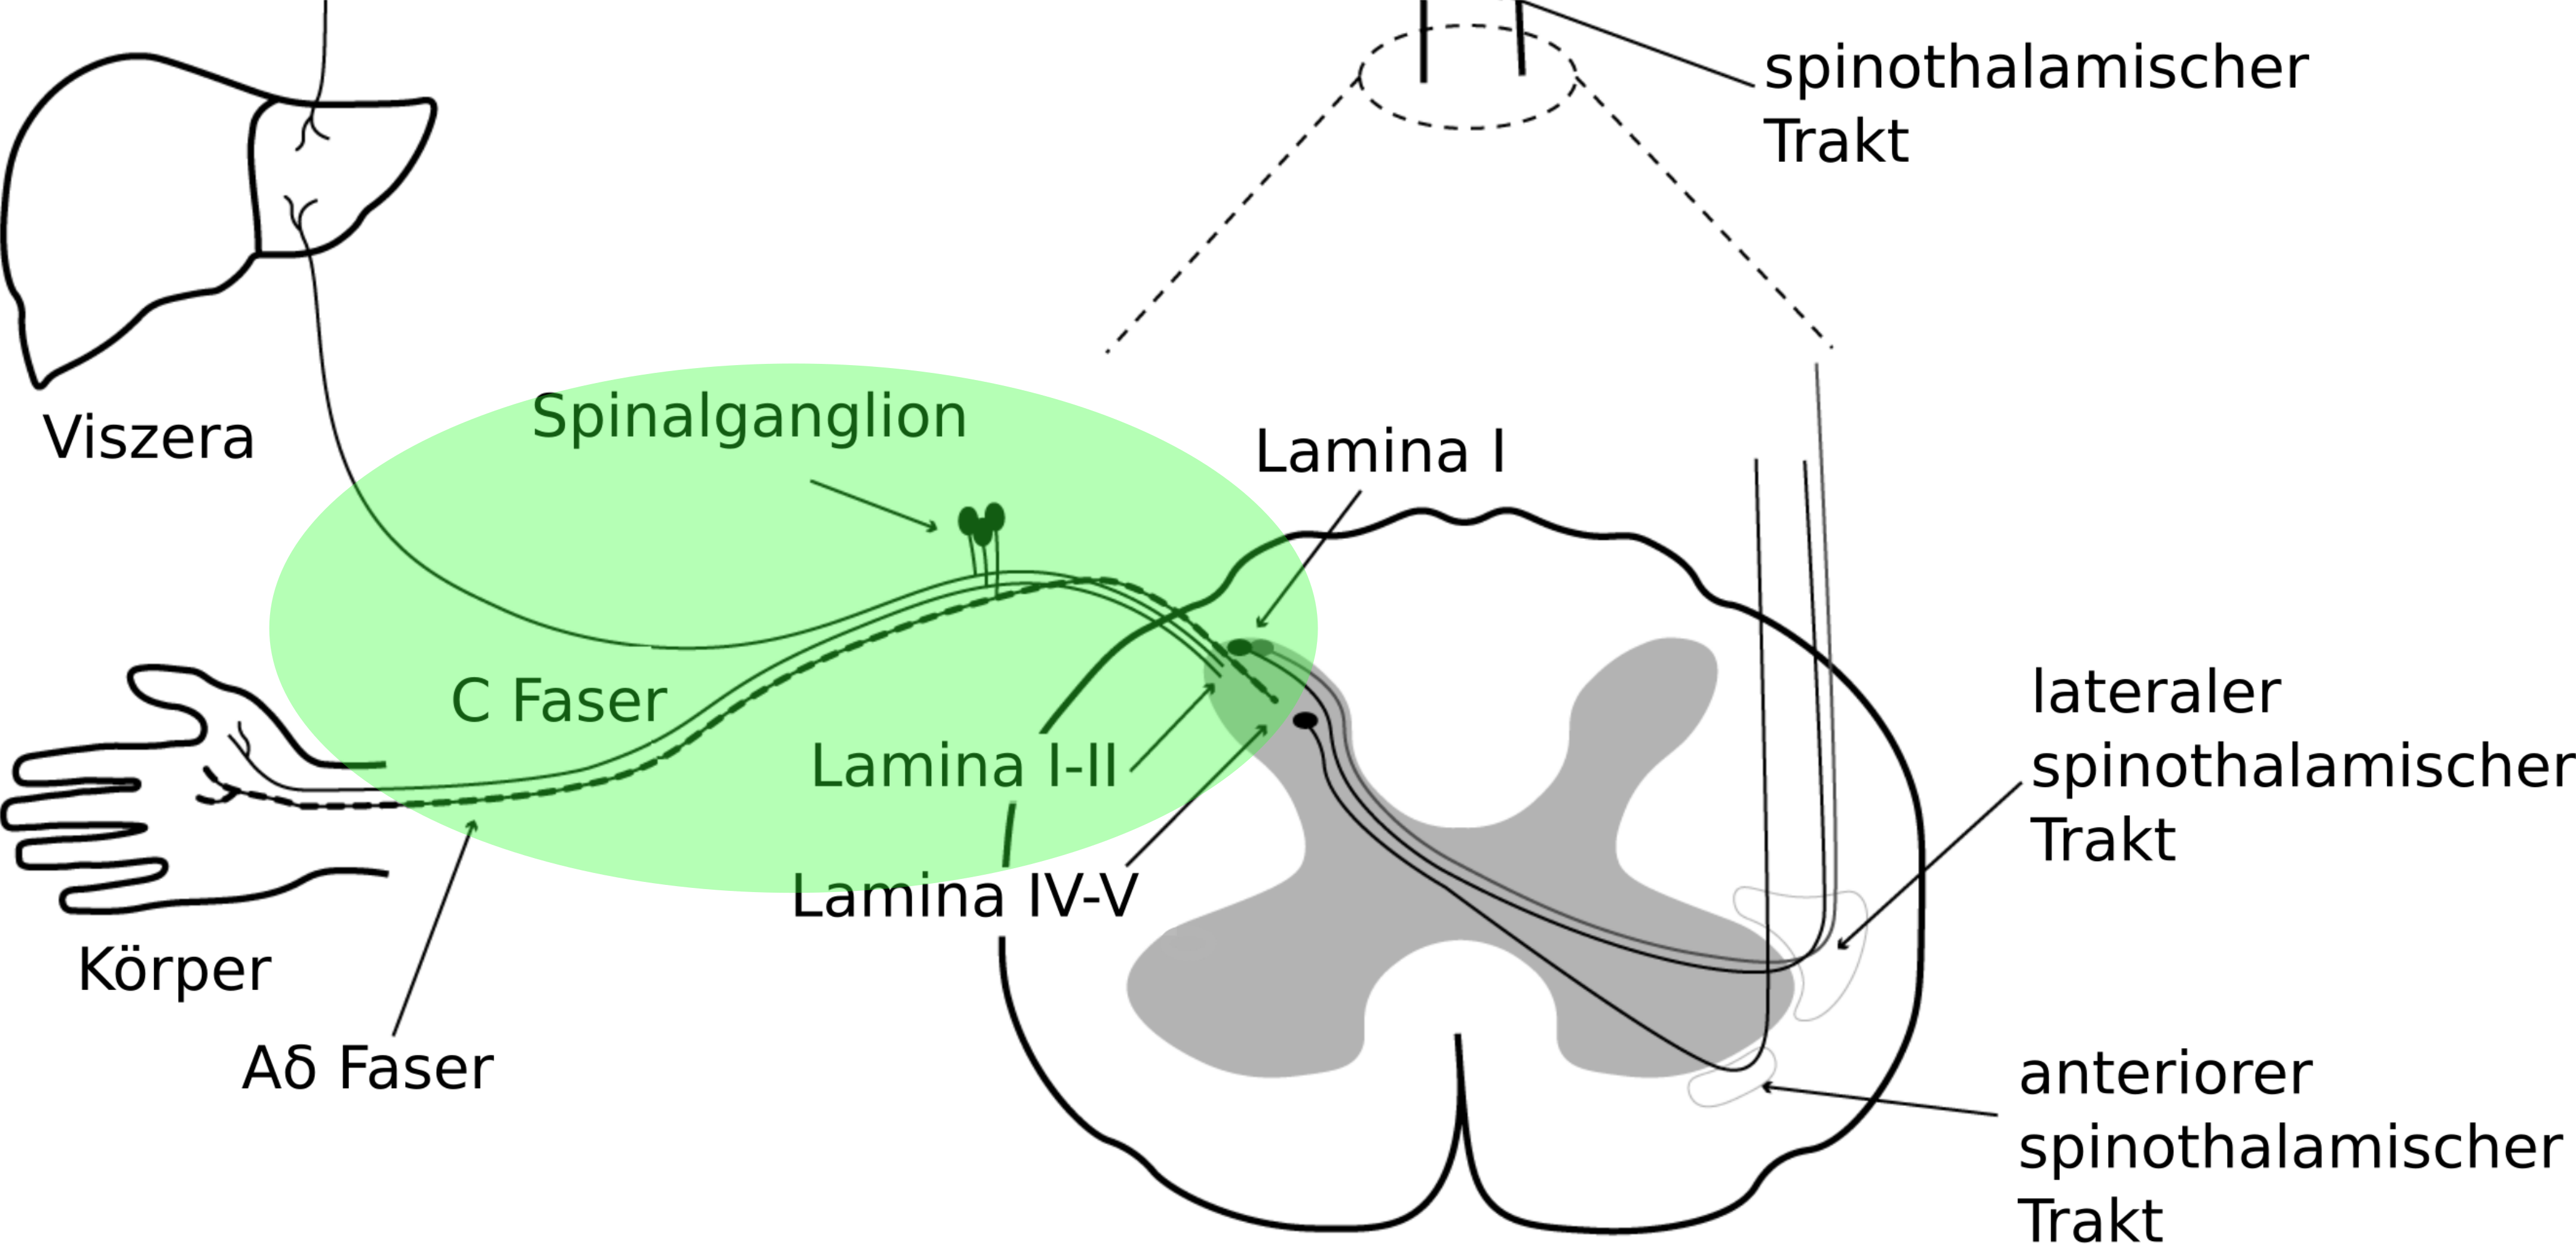
\includegraphics[width=\textwidth]{/home/melanie/Work/pictures/brain/Schmerz_aufsteigend_bis_Rueckenmark_Fasern.png}
\end{center}

Der Schmerz wird ins Rückenmark weitergeleitet über A\(\delta\) (``A delta'') oder C Fasern. 

\end{frame}

\begin{frame}
\frametitle{Schneller und langsamer Schmerz}

\begin{center}

\begin{tabular}{|l|l|}
\hline
Schneller Schmerz       & Langsamer Schmerz \\
\hline
A\(\delta\) Fasern     & C Fasern \\
(myelinisiert)          & (nicht myelinisiert) \\
6-30 m/s                & 0.5-2 m/s \\
``scharf''              & ``dumpf'' \\
\hline
\end{tabular}

\end{center}


\pause
\begin{center}
\includegraphics[width=0.5\textwidth]{/home/melanie/Work/pictures/physiology/Joe_Thomas_and_Simone_Biles.jpg}
\end{center}



\end{frame}









%% Spinal cord - dorsales Horn, vorderseitenstrang Pathway, chirurgische Eingriffe
\begin{frame}
\frametitle{Umschaltung im Rückenmark}

\begin{center}
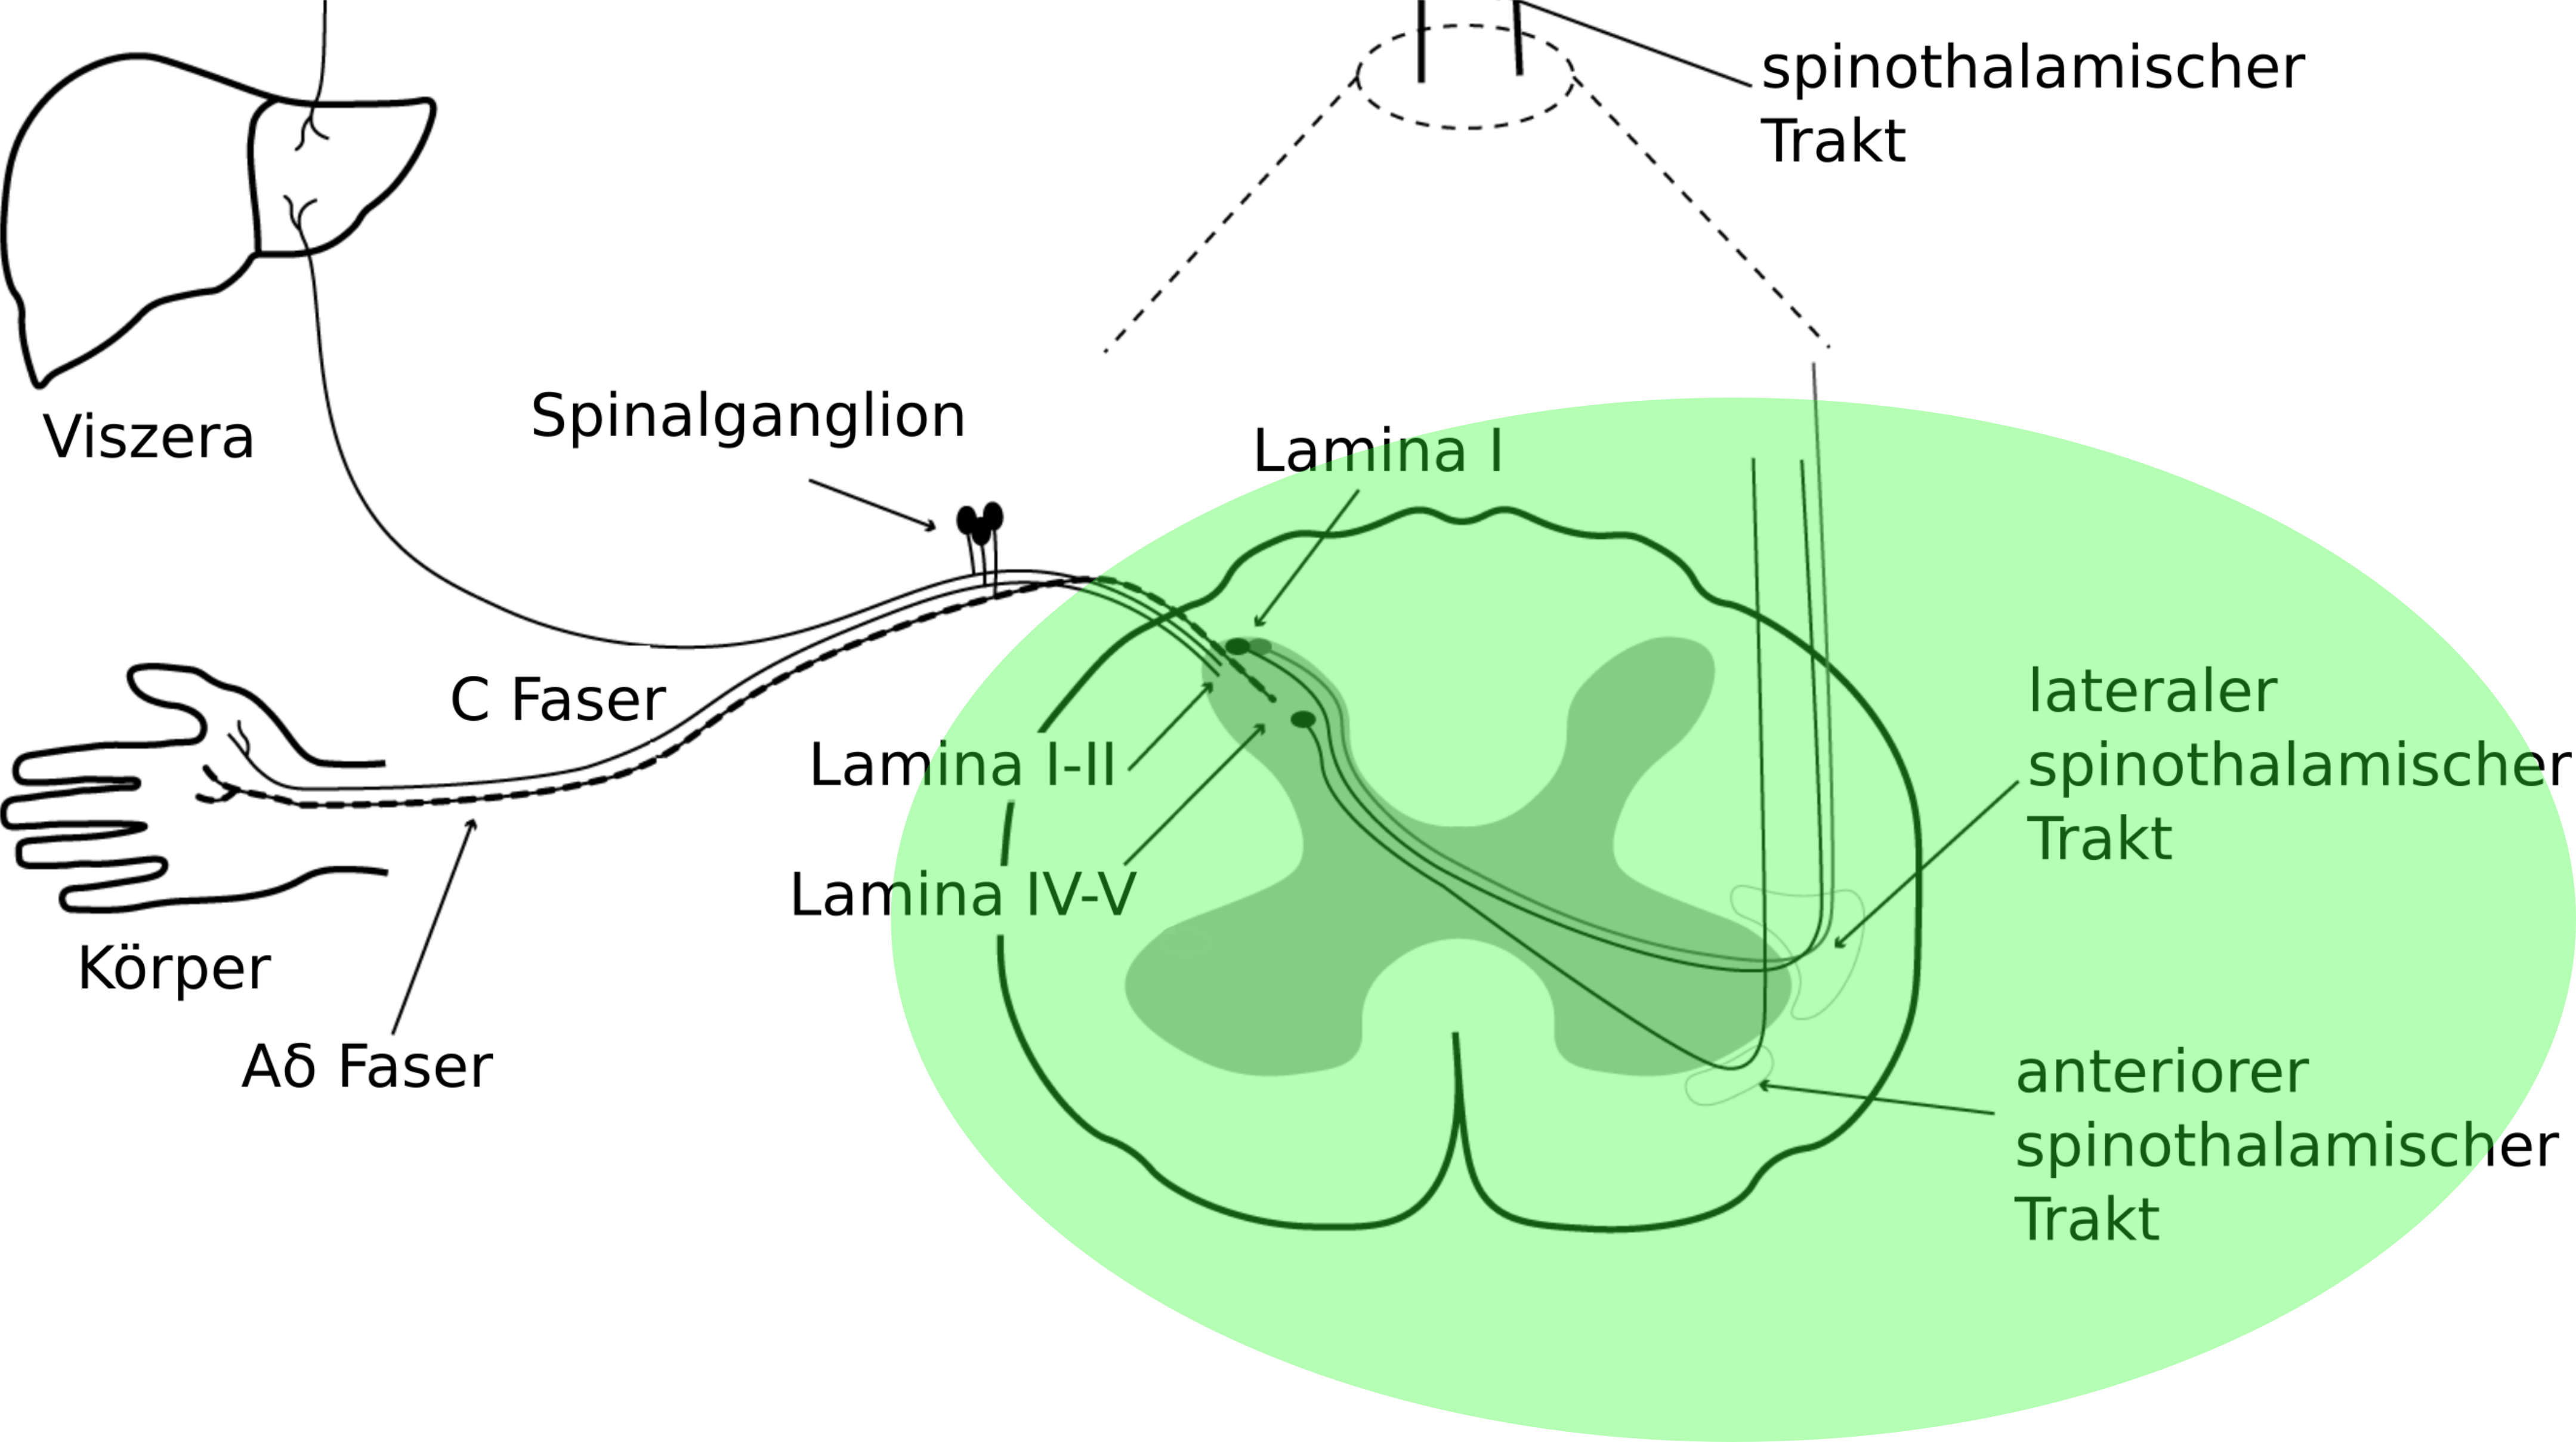
\includegraphics[width=0.8\textwidth]{/home/melanie/Work/pictures/brain/Schmerz_aufsteigend_bis_Rueckenmark_Rueckenmark.png}
\end{center}

\pause

Schmerzfasern kommen durch das Rückenhorn ins Rückenmark. Hier wird das Schmerzsignal umgeschalten (diagonal nach vorne). Es geht von dort in den Thalamus durch den tractus spinothalamicus (Vorderseitenstrang). 

\end{frame}


\begin{frame}

\frametitle{Viszeraler Schmerz}

 \begin{center}
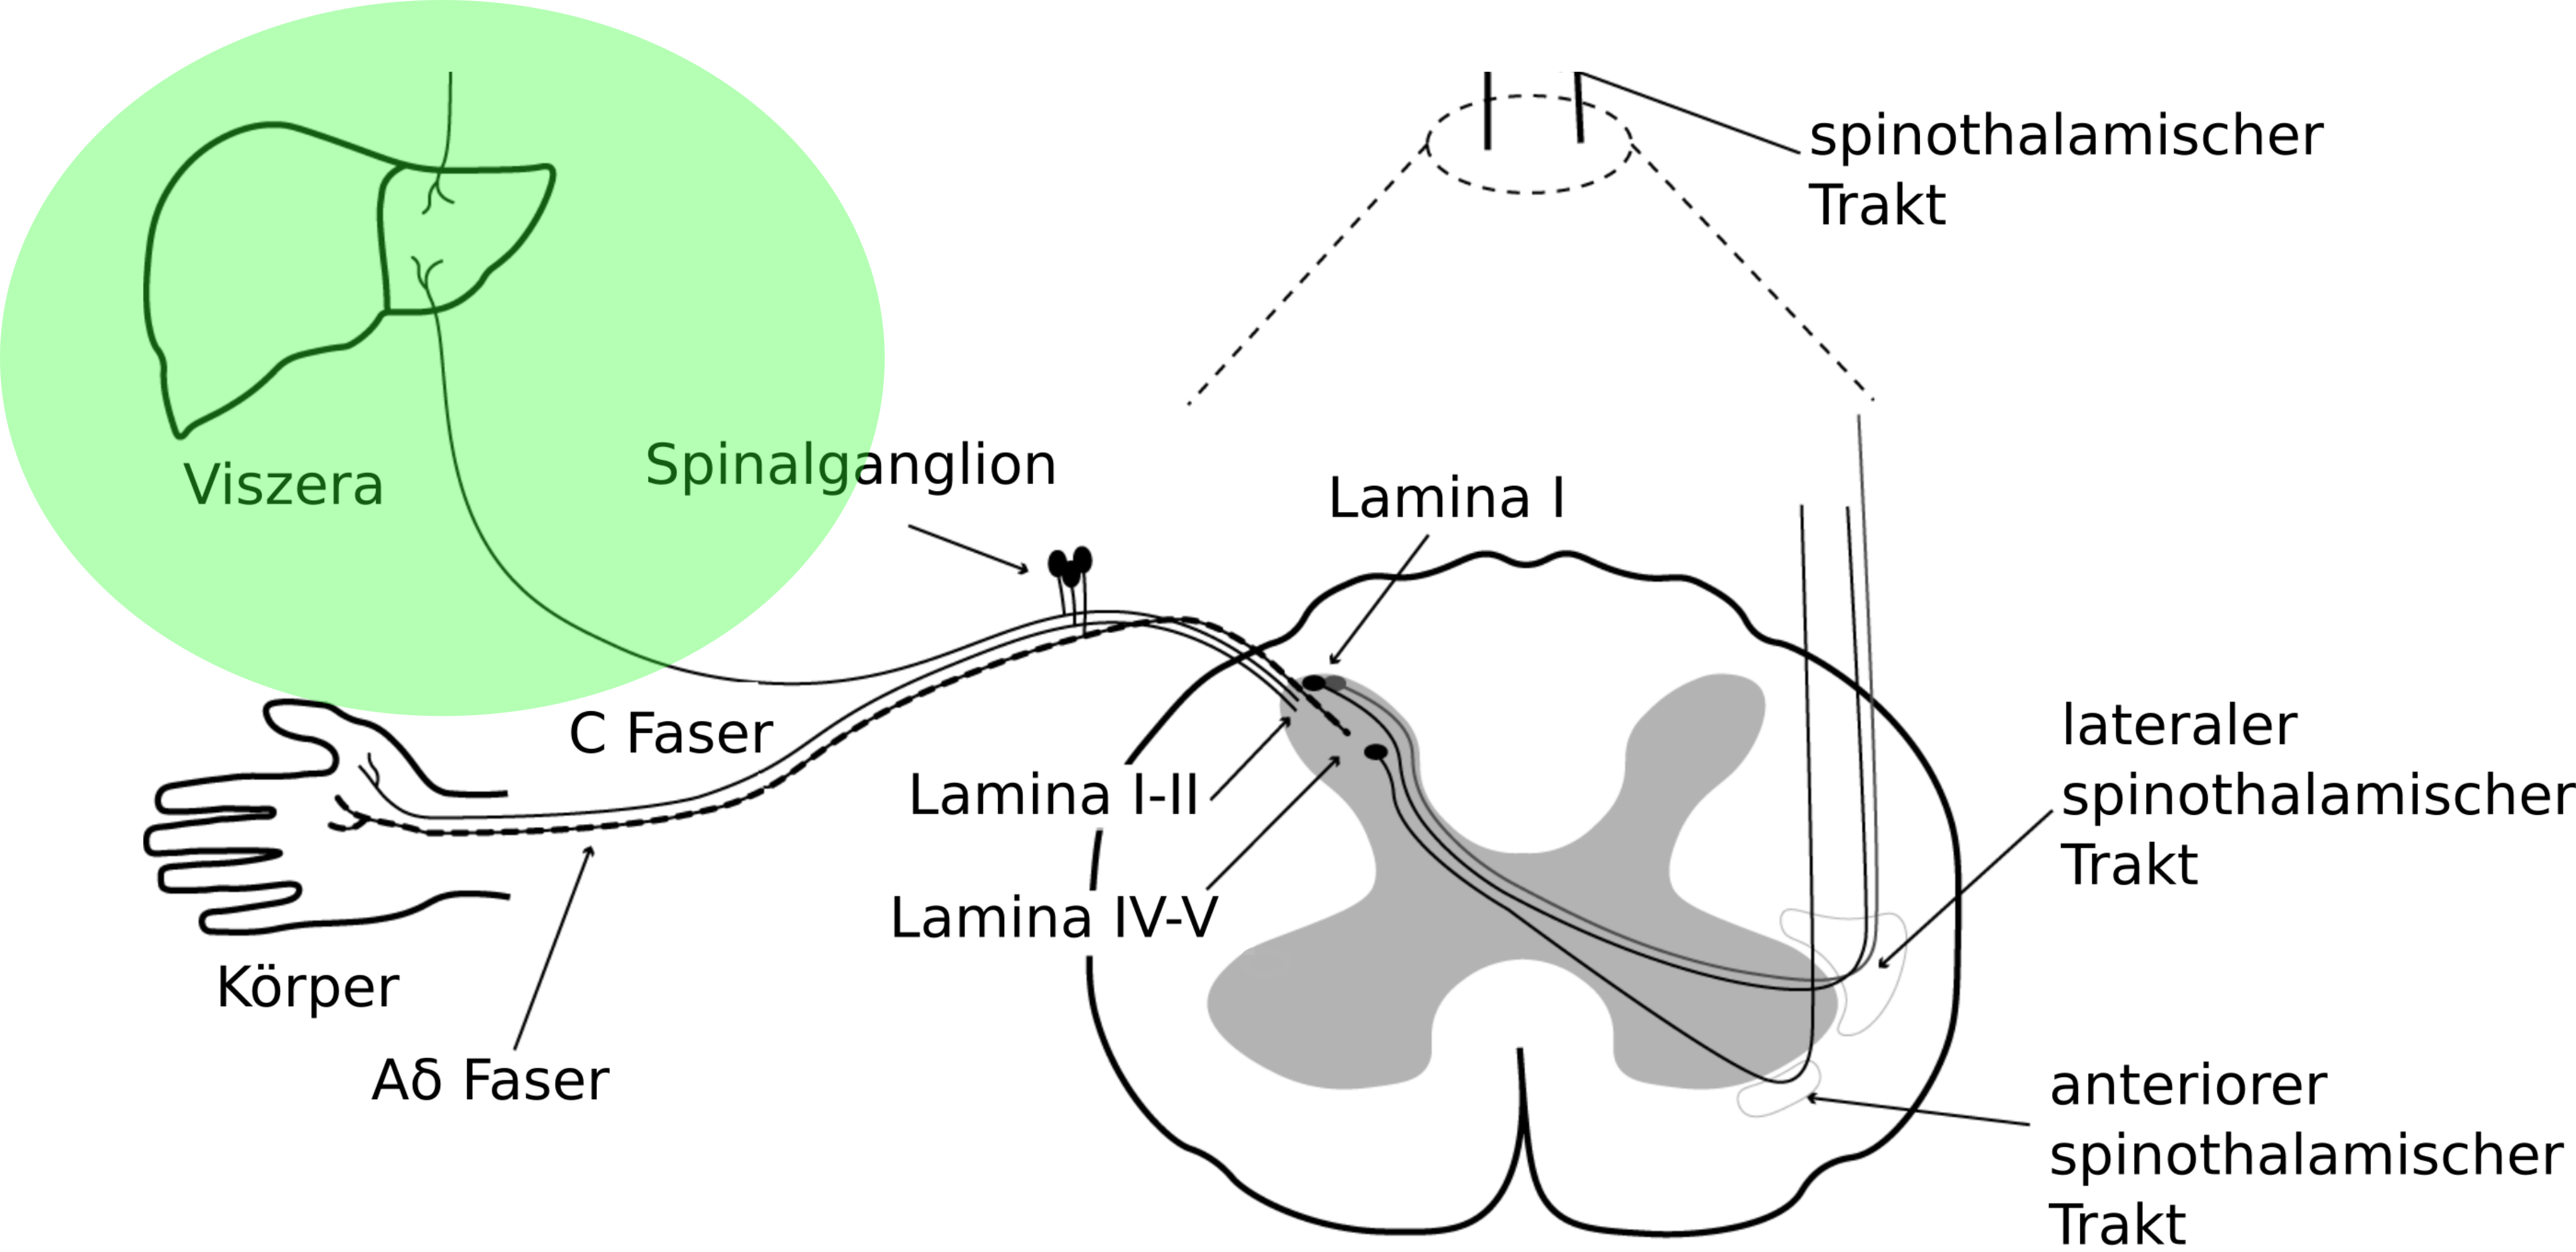
\includegraphics[width=\textwidth]{/home/melanie/Work/pictures/brain/Schmerz_aufsteigend_bis_Rueckenmark_Viszera.png}
\end{center}


\end{frame}

%% Viszeraler Schmerz - Head-Zonen  
\begin{frame}
\frametitle{Viszeraler Schmerz}

\begin{columns}[c]


\begin{column}{5cm}
Schmerzen in Eingeweiden (Viszera) entstehen oft durch
 
\begin{itemize}
\item
Verformung
\item
Ischämie (Unterdurchblutung)
\item
Entzündung
\end{itemize}
\end{column}

\begin{column}{5cm}
\begin{center}
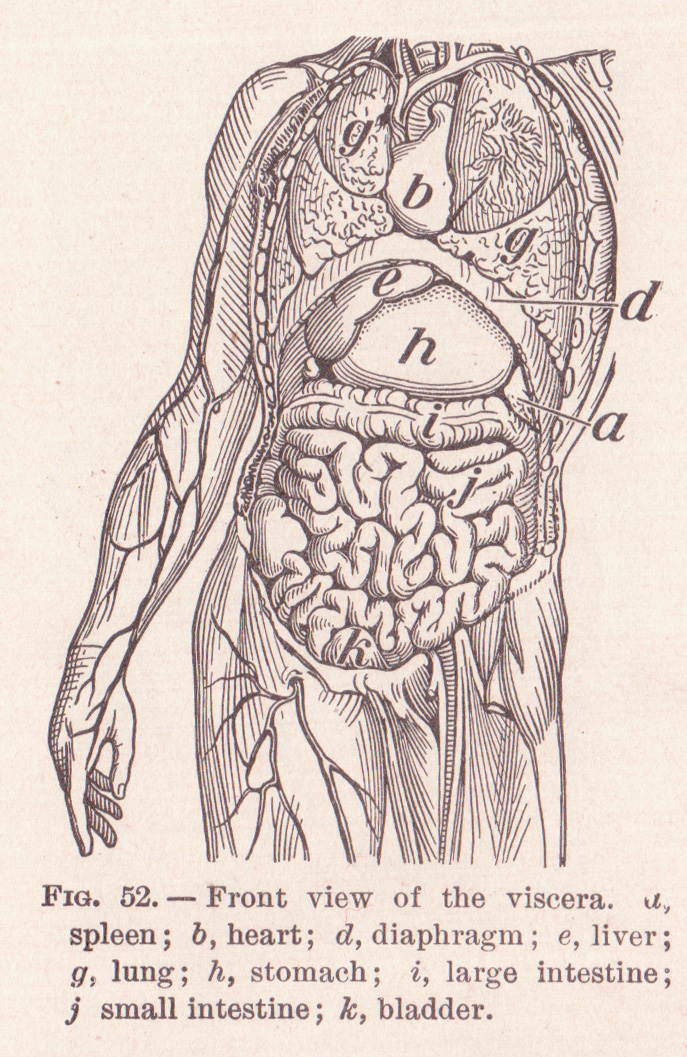
\includegraphics[width=\textwidth]{/home/melanie/Work/pictures/physiology/viscera.jpg}
\end{center}

\end{column}

\end{columns}


\end{frame}

\begin{frame}
\frametitle{Übertragener Schmerz}

Viszeraler Schmerz wird oft als Oberflächenschmerz in anderen Regionen des Körpers wahrgenommen (``übertragener Schmerz'') \\
Die Entsprechungen sind als ``Head-Zonen'' (auch ``Head'sche Zonen'') kartiert.


\begin{center}
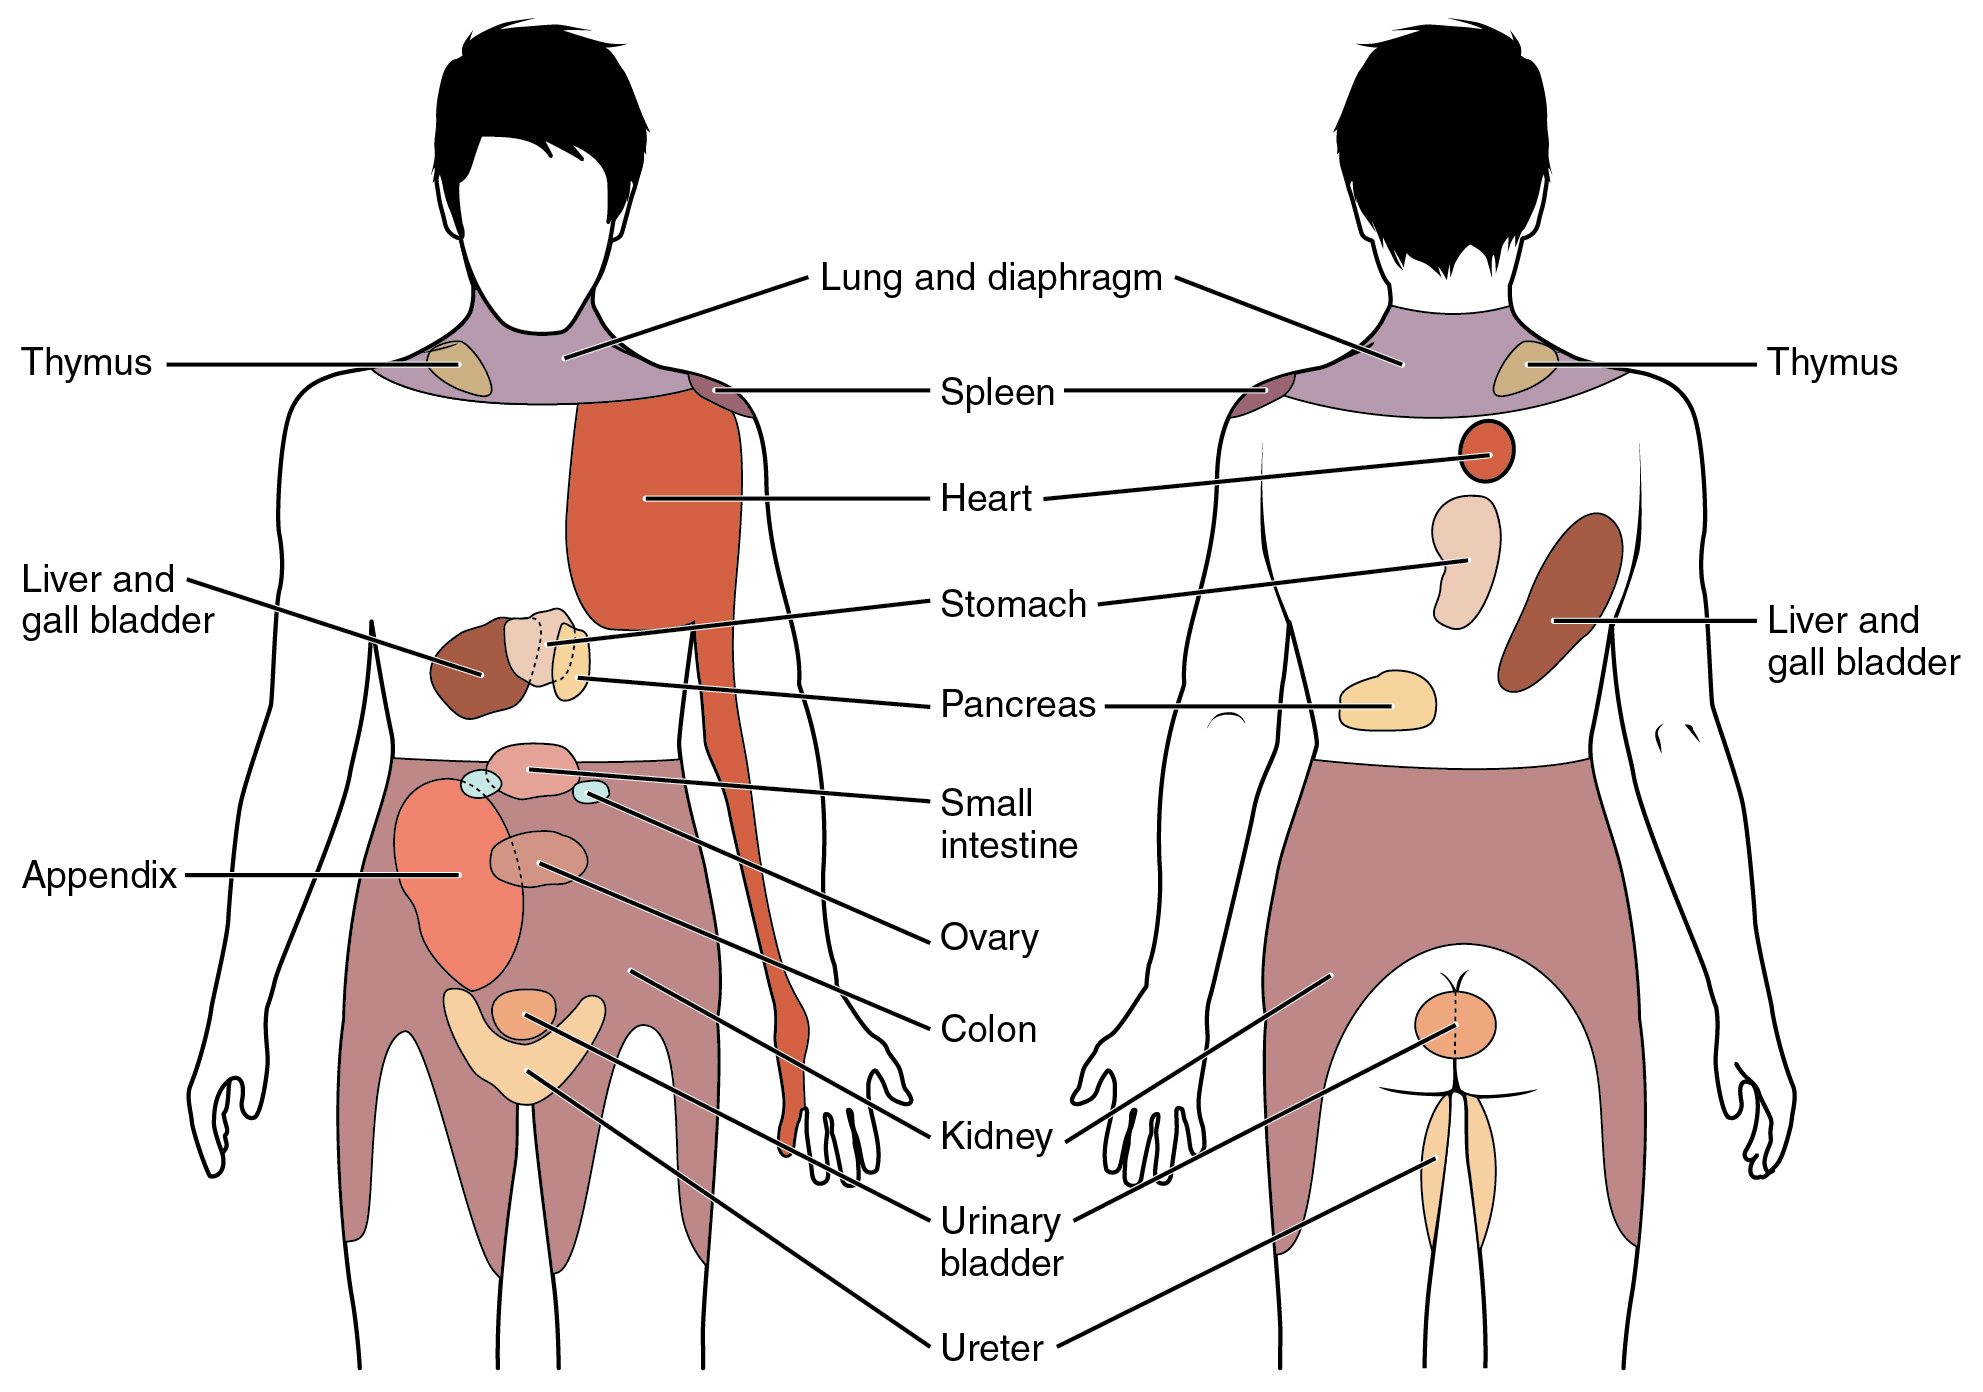
\includegraphics[width=0.7\textwidth]{/home/melanie/Work/pictures/physiology/Referred_Pain_Chart.jpg}
\end{center}

\end{frame}

\begin{frame}
\frametitle{Übertragener Schmerz}

OK \dots Aber warum? 


\pause

Mögliche Erklärung: Konvergenz im Rückenmark: Schmerzfasern aus den Viszera und aus den entsprechenden Haut-Regionen schalten im Rückenmark auf dieselben weiterleitenden Nervenfasern um. \\


\begin{center}
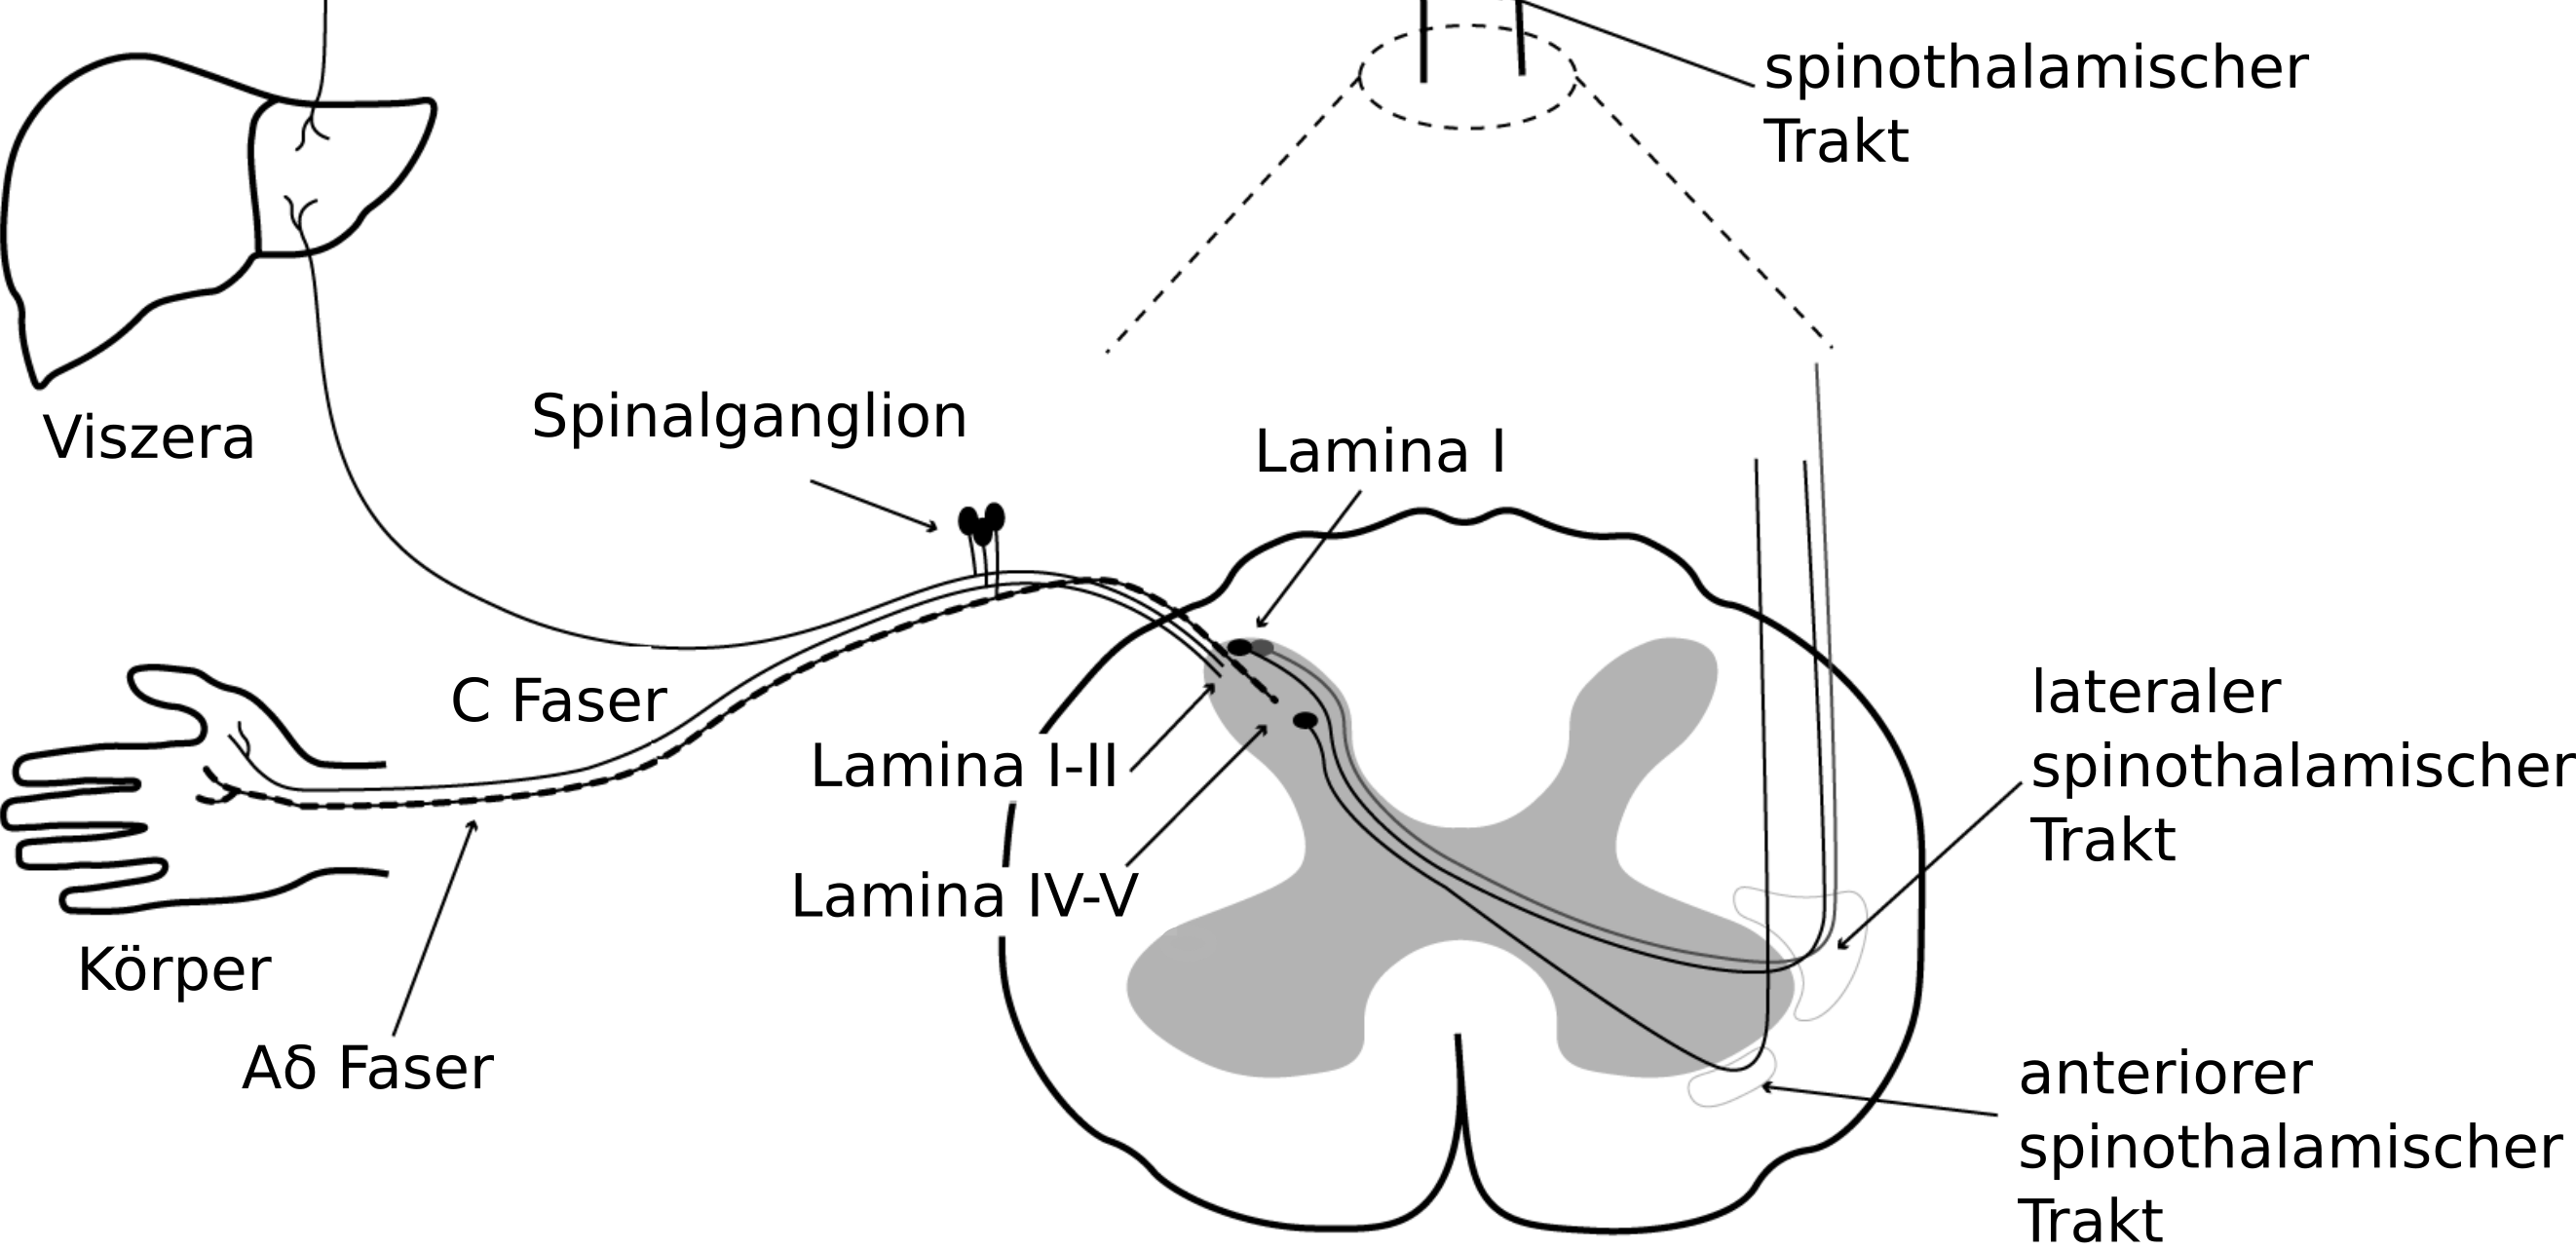
\includegraphics[width=\textwidth]{/home/melanie/Work/pictures/brain/Schmerz_aufsteigend_bis_Rueckenmark.png}
\end{center}



\end{frame}



   %% Big picture Überblick
\begin{frame}
\frametitle{Zusammenfassung}

\begin{center}
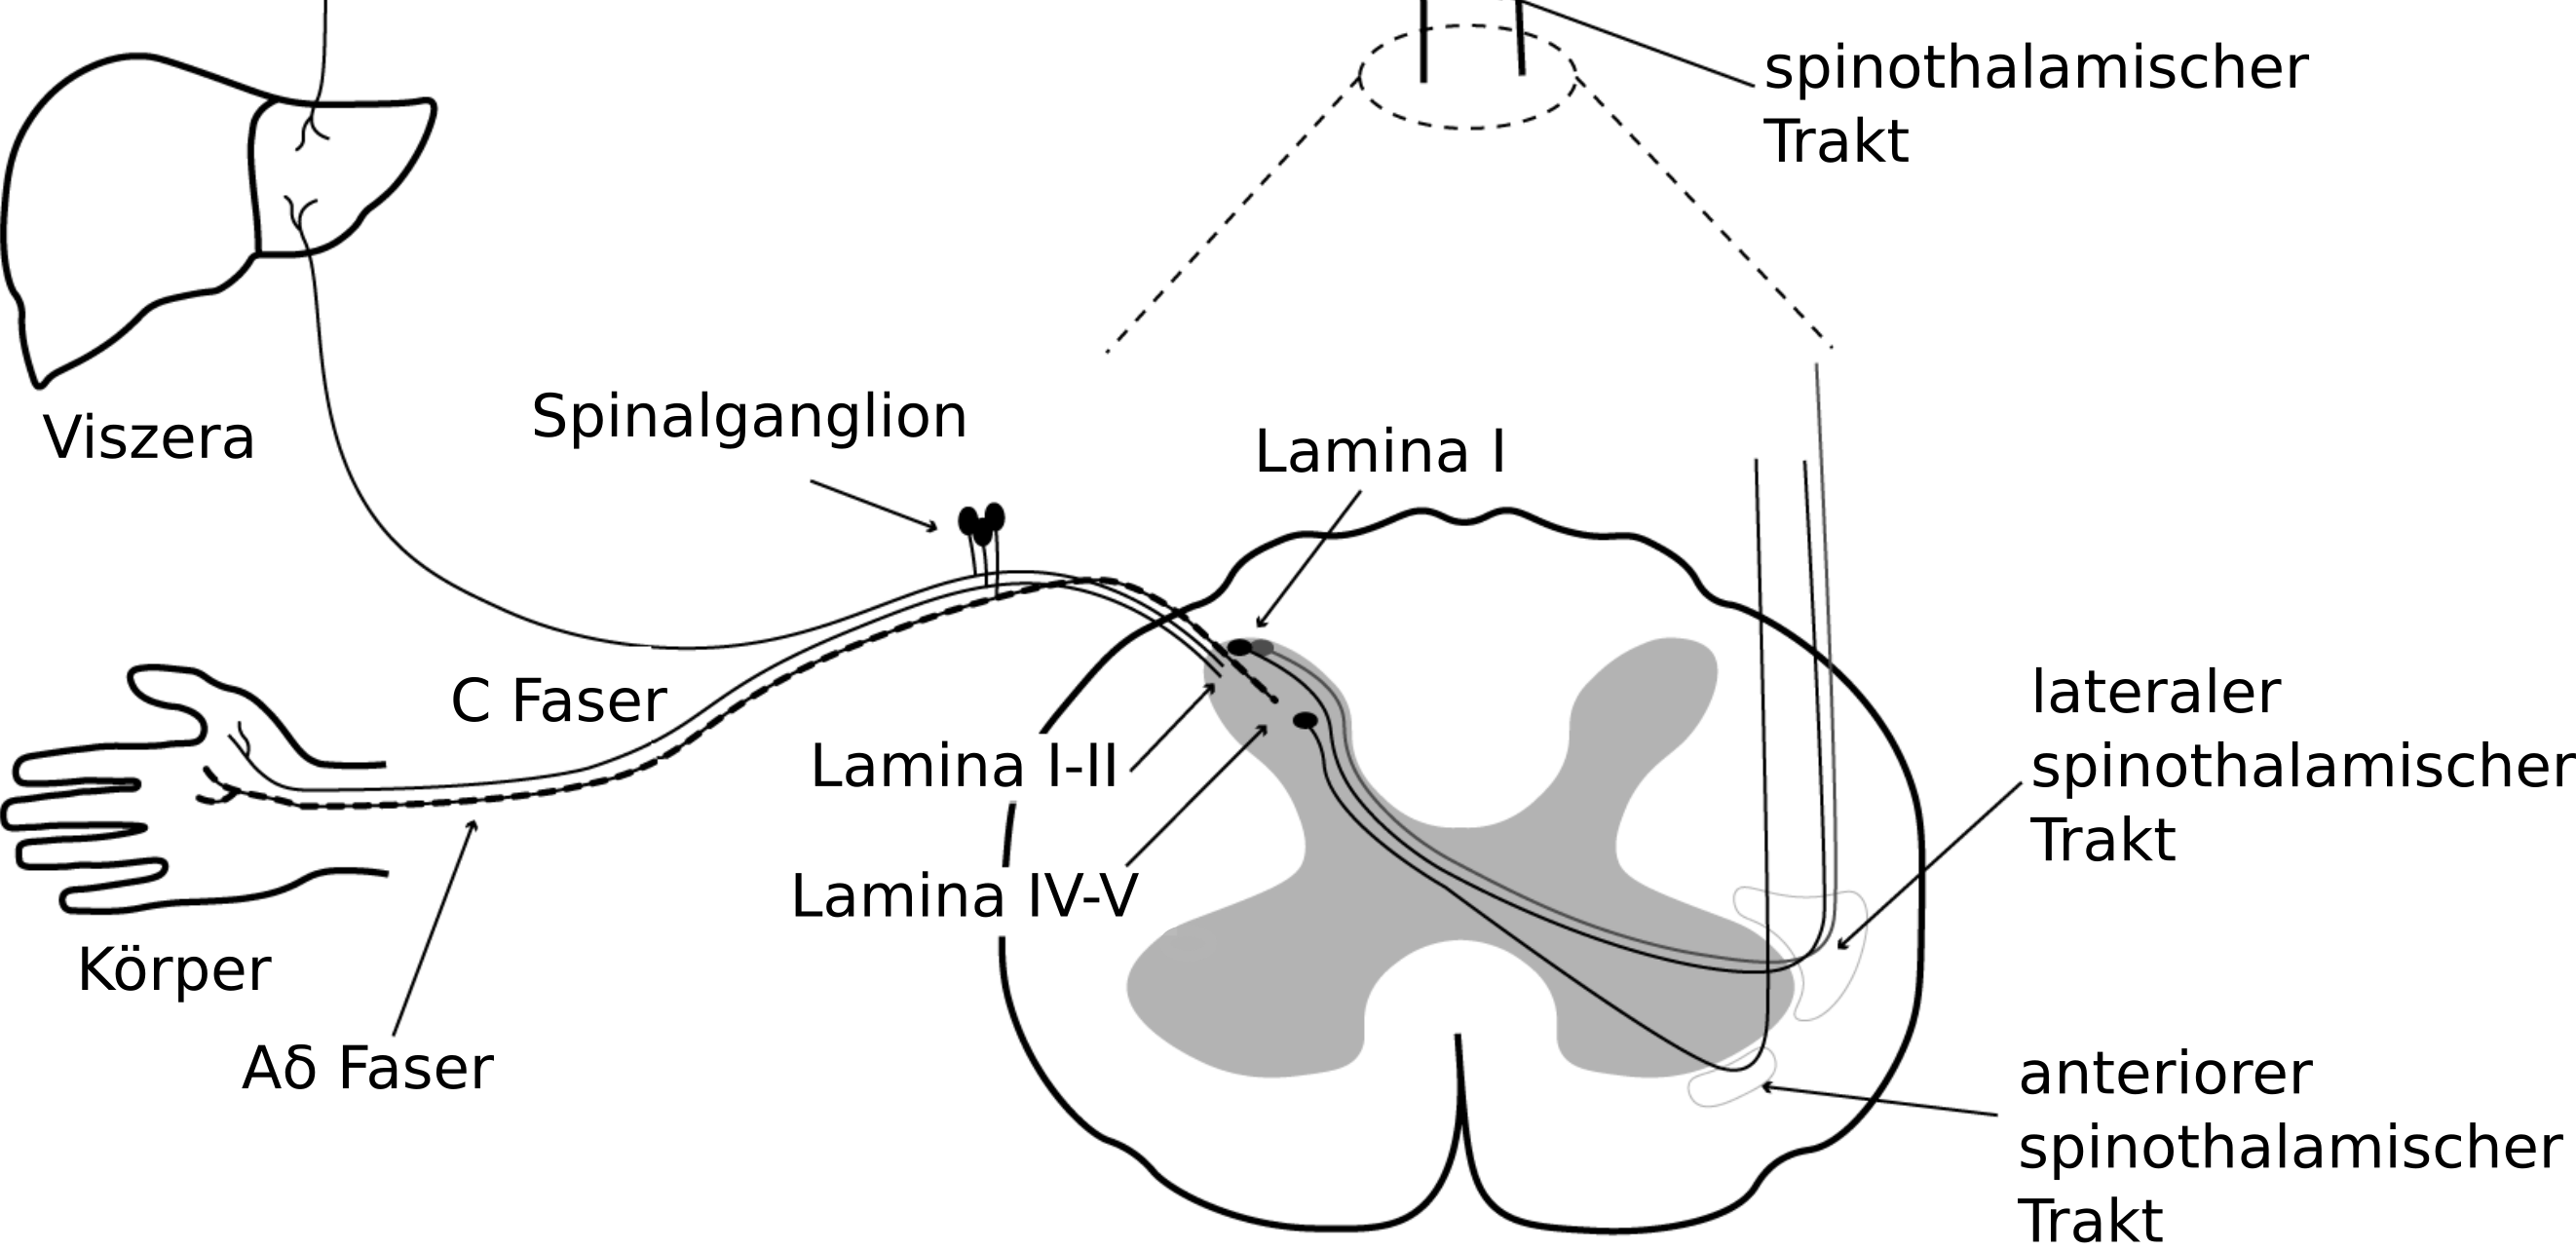
\includegraphics[width=\textwidth]{/home/melanie/Work/pictures/brain/Schmerz_aufsteigend_bis_Rueckenmark.png}
\end{center}

\end{frame}


\begin{frame}
\frametitle{Wie geht es weiter?}

\begin{center}
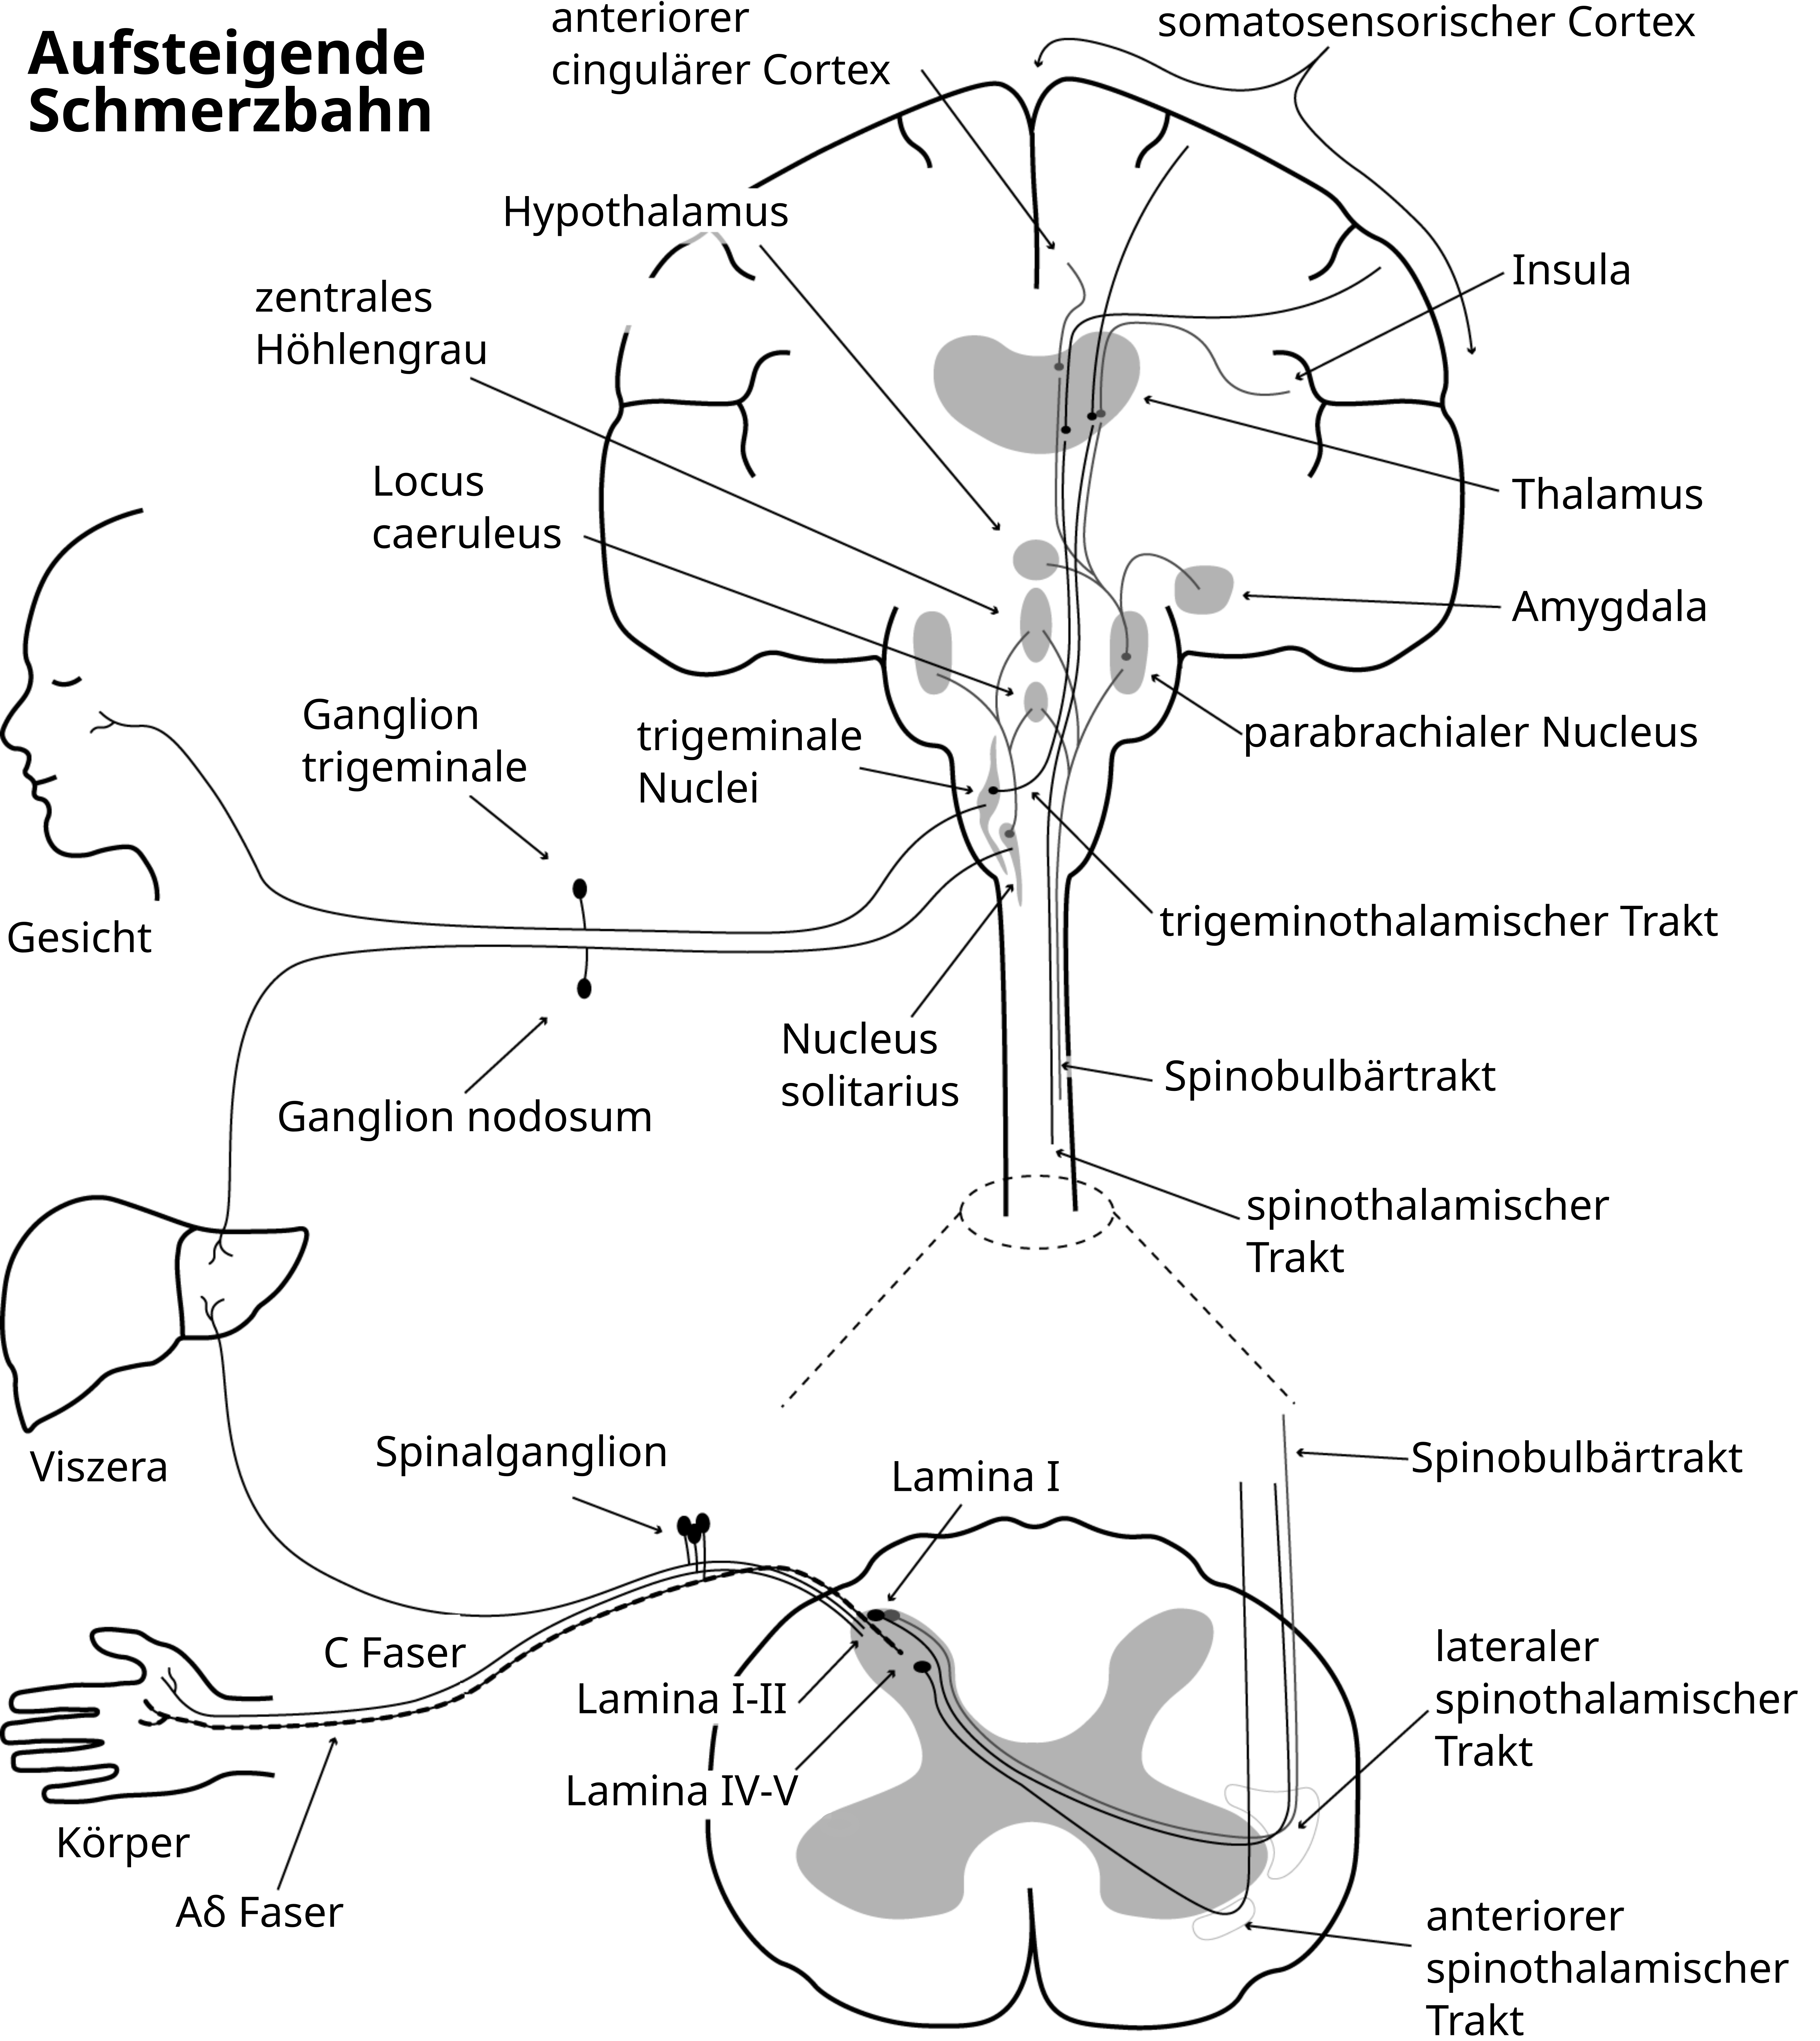
\includegraphics[width=0.5\textwidth]{/home/melanie/Work/pictures/brain/Schmerz_aufsteigend.png}
\end{center}

\end{frame}





\begin{frame}
\frametitle{Welche der Fragen vom Anfang haben wir beantwortet?}

\begin{itemize}
\item
Warum ist auf Sonnenbrand alles schmerzhaft, sogar ein T-Shirt?
\item
Wie funktioniert eigentlich Aspirin? 
\item
Warum können Schmerzen im Arm ein Anzeichen von Herzinfarkt sein? 
\item
Warum kann man bei Schmerzen schlecht schlafen? 
\item
Warum tut es weh, besonders scharfe Chilis zu essen?
\item
Warum haben manche Menschen nie Schmerzen? Und andere dauernd?
\item
Warum hilft Bewegung bei Regelschmerzen? 
\item
Wie funktionieren Phantomschmerzen?  
\item
\dots 
\end{itemize}

\end{frame}



%% Auflösung: Beantwortete Fragen
\begin{frame}
\frametitle{Welche der Fragen vom Anfang haben wir beantwortet?}

\begin{itemize}
\item
\textcolor{theme}{Warum ist auf Sonnenbrand alles schmerzhaft, sogar ein T-Shirt?}
\item
\textcolor{theme}{Wie funktioniert eigentlich Aspirin?} 
\item
\textcolor{theme}{Warum können Schmerzen im Arm ein Anzeichen von Herzinfarkt sein?}
\item
Warum kann man bei Schmerzen schlecht schlafen? 
\item
\textcolor{theme}{Warum tut es weh, besonders scharfe Chilis zu essen?}
\item
Warum haben manche Menschen nie Schmerzen? Und andere dauernd?
\item
\textcolor{theme}{Warum hilft Bewegung bei Regelschmerzen?} 
\item
Wie funktionieren Phantomschmerzen?  
\item
\dots 
\end{itemize}

\end{frame}



%% Review
 \begin{frame}
\frametitle{Lernziel-Check}


\begin{block}{Jetzt sollten Sie folgendes können:}



\begin{itemize}
\item
Den allgemeinen Weg des Schmerzreizes vom Nozizeptor bis ins Gehirn beschreiben
\item
Die drei Arten von Nozizeption aufzählen und beschreiben
\item
Erklären, wie Schmerz-Rezeptoren aktiviert werden
\item
Modifikatoren von Schmerz-Rezeptoren benennen und erklären
\item
Erklären, was schnellen von langsamem Schmerz unterscheidet
\item
Erklären, was übertragener Schmerz ist und wann er vorkommt
\end{itemize}


\end{block}

\pause

Welche Fragen haben Sie? 

\end{frame}





\begin{frame}
 
\frametitle{Bildnachweis}
 
\begin{tiny}
  

\begin{itemize}
\item
Head-Zonen. OpenStax College - Autonomic Reflexes and Homeostasis  \url{http://cnx.org/content/m46579/1.2/}, CC BY 3.0, \url{https://commons.wikimedia.org/w/index.php?curid=30017359}
\item
Innere Organe.  Sue Clark - Flickr: View of Viscera Page 82, Public Domain, \url{https://commons.wikimedia.org/w/index.php?curid=16128601}
\item
Ionenkanal.  Original uploader was Outslider (Paweł Tokarz) at pl.wikipedia - Transferred from pl.wikipedia to Commons by Masur using CommonsHelper., Public Domain, \url{https://commons.wikimedia.org/w/index.php?curid=5828577}
\item
Joe Thomas und Simone Biles. Erik Drost, CC BY 2.0 \url{https://creativecommons.org/licenses/by/2.0}, via Wikimedia Commons
\item
Kaktus. Photo by \href{https://unsplash.com/@earl_plannerzone?utm_source=unsplash&utm_medium=referral&utm_content=creditCopyText}{Earl Wilcox} on \href{https://unsplash.com/s/photos/pain?utm_source=unsplash&utm_medium=referral&utm_content=creditCopyText}{Unsplash}
\item
Prostaglandin-Synthese. Eigenes Bild, 2021. CC BY-SA 3.0.
\item
Schmerzleitung. Eigenes Bild, 2021, CC BY 4.0 \url{https://creativecommons.org/licenses/by/4.0} nach einem Bild von Richard Lennertz,  Wikimedia Commons
\item
Sonnenbrand. By Phil Kates - \url{https://www.flickr.com/photos/hawk684/108139247/}, CC BY-SA 2.0, \url{https://commons.wikimedia.org/w/index.php?curid=51031248}
\item
Substanz P. Fvasconcellos - Own work, Public Domain, \url{https://commons.wikimedia.org/w/index.php?curid=1017110}
\item
TRPV1. Von The Author 2011. Published by Oxford University Press - \url{https://www.ncbi.nlm.nih.gov/core/lw/2.0/html/tileshop_pmc/tileshop_pmc_inline.html?title=Click on image to zoom&p=PMC3&id=3169333_aer26002.jpg}
CC BY-SA 2.5, \url{https://commons.wikimedia.org/w/index.php?curid=34131563}
\end{itemize}

\end{tiny}

\end{frame}




\end{document}




